%&preformat-disser
\RequirePackage[l2tabu,orthodox]{nag}
\documentclass[a4paper,14pt,oneside,openany]{memoir}

%%%%%%%%%%%%%%%%%%%%%%%%%%%%%%%%%%%%%%%%%%%%%%%%%%%%%%%%%%%%%%%%%%%%%%%%%%%%%%%%
%%%% Файл упрощённых настроек шаблона, общих для диссертации и автореферата %%%%
%%%%%%%%%%%%%%%%%%%%%%%%%%%%%%%%%%%%%%%%%%%%%%%%%%%%%%%%%%%%%%%%%%%%%%%%%%%%%%%%

%%% Режим черновика %%%
\makeatletter
\@ifundefined{c@draft}{
  \newcounter{draft}
  \setcounter{draft}{0}  % 0 --- чистовик (максимальное соблюдение ГОСТ)
                         % 1 --- черновик (отклонения от ГОСТ, но быстрая
                         %       сборка итоговых PDF)
}{}
\makeatother

%%% Пометки в тексте %%%
\makeatletter
\@ifundefined{c@showmarkup}{
  \newcounter{showmarkup}
  \setcounter{showmarkup}{0}  % 0 --- скрыть пометки
                              % 1 --- показывать пометки
}{}
\makeatother

%%% Использование в pdflatex шрифтов не по-умолчанию %%%
\makeatletter
\@ifundefined{c@usealtfont}{
  \newcounter{usealtfont}
  \setcounter{usealtfont}{1}    % 0 --- шрифты на базе Computer Modern
                                % 1 --- использовать пакет pscyr, при его
                                %       наличии
                                % 2 --- использовать пакет XCharter, при наличии
                                %       подходящей версии
}{}
\makeatother

%%% Использование в xelatex и lualatex семейств шрифтов %%%
\makeatletter
\@ifundefined{c@fontfamily}{
  \newcounter{fontfamily}
  \setcounter{fontfamily}{1}  % 0 --- CMU семейство. Используется как fallback;
                              % 1 --- Шрифты от MS (Times New Roman и компания)
                              % 2 --- Семейство Liberation
}{}
\makeatother

%%% Библиография %%%
\makeatletter
\@ifundefined{c@bibliosel}{
  \newcounter{bibliosel}
  \setcounter{bibliosel}{1}   % 0 --- встроенная реализация с загрузкой файла
                              %       через движок bibtex8;
                              % 1 --- реализация пакетом biblatex через движок
                              %       biber
}{}
\makeatother

%%% Предкомпиляция tikz рисунков для ускорения работы %%%
\makeatletter
\@ifundefined{c@imgprecompile}{
  \newcounter{imgprecompile}
  \setcounter{imgprecompile}{0}   % 0 --- без предкомпиляции;
                                  % 1 --- пользоваться предварительно
                                  %       скомпилированными pdf вместо генерации
                                  %       заново из tikz
}{}
\makeatother


%%%%%%%%%%%%%%%%%%%%%%%%%%%%%%%%%%%%%%%%%%%%%%%%%%%%%%
%%%% Файл упрощённых настроек шаблона диссертации %%%%
%%%%%%%%%%%%%%%%%%%%%%%%%%%%%%%%%%%%%%%%%%%%%%%%%%%%%%

%%% Инициализирование переменных, не трогать!  %%%
\newcounter{intvl}
\newcounter{otstup}
\newcounter{contnumeq}
\newcounter{contnumfig}
\newcounter{contnumtab}
\newcounter{pgnum}
\newcounter{chapstyle}
\newcounter{headingdelim}
\newcounter{headingalign}
\newcounter{headingsize}
%%%%%%%%%%%%%%%%%%%%%%%%%%%%%%%%%%%%%%%%%%%%%%%%%%%%%%

%%% Область упрощённого управления оформлением %%%

%% Интервал между заголовками и между заголовком и текстом %%
% Заголовки отделяют от текста сверху и снизу
% тремя интервалами (ГОСТ Р 7.0.11-2011, 5.3.5)
\setcounter{intvl}{2}               % Коэффициент кратности к размеру шрифта

%% Отступы у заголовков в тексте %%
\setcounter{otstup}{1}              % 0 --- без отступа; 1 --- абзацный отступ

%% Нумерация формул, таблиц и рисунков %%
% Нумерация формул
\setcounter{contnumeq}{0}   % 0 --- пораздельно (во введении подряд,
                            %       без номера раздела);
                            % 1 --- сквозная нумерация по всей диссертации
% Нумерация рисунков
\setcounter{contnumfig}{0}  % 0 --- пораздельно (во введении подряд,
                            %       без номера раздела);
                            % 1 --- сквозная нумерация по всей диссертации
% Нумерация таблиц
\setcounter{contnumtab}{1}  % 0 --- пораздельно (во введении подряд,
                            %       без номера раздела);
                            % 1 --- сквозная нумерация по всей диссертации

%% Оглавление %%
\setcounter{pgnum}{1}       % 0 --- номера страниц никак не обозначены;
                            % 1 --- Стр. над номерами страниц (дважды
                            %       компилировать после изменения настройки)
\settocdepth{subsection}    % до какого уровня подразделов выносить в оглавление
\setsecnumdepth{subsection} % до какого уровня нумеровать подразделы


%% Текст и форматирование заголовков %%
\setcounter{chapstyle}{1}     % 0 --- разделы только под номером;
                              % 1 --- разделы с названием "Глава" перед номером
\setcounter{headingdelim}{0}  % 0 --- номер отделен пропуском в 1em или \quad;
                              % 1 --- номера разделов и приложений отделены
                              %       точкой с пробелом, подразделы пропуском
                              %       без точки;
                              % 2 --- номера разделов, подразделов и приложений
                              %       отделены точкой с пробелом.

%% Выравнивание заголовков в тексте %%
\setcounter{headingalign}{0}  % 0 --- по центру;
                              % 1 --- по левому краю

%% Размеры заголовков в тексте %%
\setcounter{headingsize}{0}   % 0 --- по ГОСТ, все всегда 14 пт;
                              % 1 --- пропорционально изменяющийся размер
                              %       в зависимости от базового шрифта

%% Подпись таблиц %%

% Смещение строк подписи после первой строки
\newcommand{\tabindent}{0cm}

% Тип форматирования заголовка таблицы:
% plain --- название и текст в одной строке
% split --- название и текст в разных строках
\newcommand{\tabformat}{plain}

%%% Настройки форматирования таблицы `plain`

% Выравнивание по центру подписи, состоящей из одной строки:
% true  --- выравнивать
% false --- не выравнивать
\newcommand{\tabsinglecenter}{false}

% Выравнивание подписи таблиц:
% justified   --- выравнивать как обычный текст («по ширине»)
% centering   --- выравнивать по центру
% centerlast  --- выравнивать по центру только последнюю строку
% centerfirst --- выравнивать по центру только первую строку (не рекомендуется)
% raggedleft  --- выравнивать по правому краю
% raggedright --- выравнивать по левому краю
\newcommand{\tabjust}{justified}

% Разделитель записи «Таблица #» и названия таблицы
\newcommand{\tablabelsep}{~\cyrdash\ }

%%% Настройки форматирования таблицы `split`

% Положение названия таблицы:
% \centering   --- выравнивать по центру
% \raggedleft  --- выравнивать по правому краю
% \raggedright --- выравнивать по левому краю
\newcommand{\splitformatlabel}{\raggedleft}

% Положение текста подписи:
% \centering   --- выравнивать по центру
% \raggedleft  --- выравнивать по правому краю
% \raggedright --- выравнивать по левому краю
\newcommand{\splitformattext}{\raggedright}

%% Подпись рисунков %%
%Разделитель записи «Рисунок #» и названия рисунка
\newcommand{\figlabelsep}{~\cyrdash\ }  % (ГОСТ 2.105, 4.3.1)
                                        % "--- здесь не работает
            % общие настройки шаблона
%%% Проверка используемого TeX-движка %%%
\newif\ifxetexorluatex   % определяем новый условный оператор (http://tex.stackexchange.com/a/47579)
\ifxetex
    \xetexorluatextrue
\else
    \ifluatex
        \xetexorluatextrue
    \else
        \xetexorluatexfalse
    \fi
\fi

\newif\ifsynopsis           % Условие, проверяющее, что документ --- автореферат

\usepackage{etoolbox}[2015/08/02]   % Для продвинутой проверки разных условий
\providebool{presentation}
\usepackage{graphicx}
\usepackage{comment}    % Позволяет убирать блоки текста (добавляет
                        % окружение comment и команду \excludecomment)

%%% Поля и разметка страницы %%%
\usepackage{pdflscape}  % Для включения альбомных страниц
\usepackage{geometry}   % Для последующего задания полей

%%% Математические пакеты %%%
\usepackage{amsthm,amsmath,amscd}   % Математические дополнения от AMS
\usepackage{amsfonts,amssymb}       % Математические дополнения от AMS
\usepackage{mathtools}              % Добавляет окружение multlined
\usepackage{xfrac}                  % Красивые дроби
\usepackage[
    locale = DE,
    list-separator       = {;\,},
    list-final-separator = {;\,},
    list-pair-separator  = {;\,},
    range-phrase={\text{\ensuremath{-}}},
    % quotient-mode        = fraction, % красивые дроби могут не соответствовать ГОСТ
    fraction-function    = \sfrac,
    separate-uncertainty,
    ]{siunitx}                      % Размерности SI
\sisetup{inter-unit-product = \ensuremath{{}\cdot{}}}

% Кириллица в нумерации subequations
% Для правильной работы требуется выполнение сразу после загрузки пакетов
\patchcmd{\subequations}{\def\theequation{\theparentequation\alph{equation}}}
{\def\theequation{\theparentequation\asbuk{equation}}}
{\typeout{subequations patched}}{\typeout{subequations not patched}}

%%%% Установки для размера шрифта 14 pt %%%%
%% Формирование переменных и констант для сравнения (один раз для всех подключаемых файлов)%%
%% должно располагаться до вызова пакета fontspec или polyglossia, потому что они сбивают его работу
\newlength{\curtextsize}
\newlength{\bigtextsize}
\setlength{\bigtextsize}{13.9pt}

\makeatletter
%\show\f@size    % неплохо для отслеживания, но вызывает стопорение процесса,
                 % если документ компилируется без команды  -interaction=nonstopmode
\setlength{\curtextsize}{\f@size pt}
\makeatother

%%% Кодировки и шрифты %%%
\ifxetexorluatex
    \PassOptionsToPackage{no-math}{fontspec}    % https://tex.stackexchange.com/a/26295/104425
    \usepackage{polyglossia}[2014/05/21]        % Поддержка многоязычности
                                        % (fontspec подгружается автоматически)
\else
   %%% Решение проблемы копирования текста в буфер кракозябрами
    \ifnumequal{\value{usealtfont}}{0}{}{
        \input glyphtounicode.tex
        \input glyphtounicode-cmr.tex %from pdfx package
        \pdfgentounicode=1
    }
    \usepackage{cmap}   % Улучшенный поиск русских слов в полученном pdf-файле
    \ifnumequal{\value{usealtfont}}{2}{}{
        \defaulthyphenchar=127  % Если стоит до fontenc, то переносы
                                % не впишутся в выделяемый текст при
                                % копировании его в буфер обмена
    }
    \usepackage{textcomp}
    \usepackage[T1,T2A]{fontenc}                    % Поддержка русских букв
    \ifnumequal{\value{usealtfont}}{1}{% Используется pscyr, при наличии
        \IfFileExists{pscyr.sty}{\usepackage{pscyr}}{}  % Подключение pscyr
    }{}
    \usepackage[utf8]{inputenc}[2014/04/30]         % Кодировка utf8
    \usepackage[english, ukrainian]{babel}[2014/03/24]% Языки: русский, английский
    \makeatletter\AtBeginDocument{\let\@elt\relax}\makeatother % babel 3.40 fix
    \ifnumequal{\value{usealtfont}}{2}{
        % http://dxdy.ru/post1238763.html#p1238763
        \usepackage[scaled=0.960]{XCharter}[2017/12/19] % Подключение русифицированных шрифтов XCharter
        \usepackage[charter, vvarbb, scaled=1.048]{newtxmath}[2017/12/14]
        \ifpresentation
        \else
            \setDisplayskipStretch{-0.078}
        \fi
    }{}
\fi

%%% Оформление абзацев %%%
\ifpresentation
\else
    \indentafterchapter     % Красная строка после заголовков типа chapter
\fi

%%% Цвета %%%
\ifpresentation
\else
    \usepackage[dvipsnames, table, hyperref]{xcolor} % Совместимо с tikz
\fi

%%% Таблицы %%%
\usepackage{longtable,ltcaption} % Длинные таблицы
\usepackage{multirow,makecell}   % Улучшенное форматирование таблиц
\usepackage{tabu, tabulary}      % таблицы с автоматически подбирающейся
                                 % шириной столбцов (tabu обязательно
                                 % до hyperref вызывать)
\usepackage{threeparttable}      % автоматический подгон ширины подписи таблицы

%%% Общее форматирование
\usepackage{soulutf8}% Поддержка переносоустойчивых подчёркиваний и зачёркиваний
\usepackage{icomma}  % Запятая в десятичных дробях

%%% Оптимизация расстановки переносов и длины последней строки абзаца
\IfFileExists{impnattypo.sty}{% проверка установленности пакета impnattypo
    \ifluatex
        \ifnumequal{\value{draft}}{1}{% Черновик
            \usepackage[hyphenation, lastparline, nosingleletter, homeoarchy,
            rivers, draft]{impnattypo}
        }{% Чистовик
            \usepackage[hyphenation, lastparline, nosingleletter]{impnattypo}
        }
    \else
        \usepackage[hyphenation, lastparline]{impnattypo}
    \fi
}{}

%% Векторная графика

\usepackage{tikz}                   % Продвинутый пакет векторной графики
\usetikzlibrary{chains}             % Для примера tikz рисунка
\usetikzlibrary{shapes.geometric}   % Для примера tikz рисунка
\usetikzlibrary{shapes.symbols}     % Для примера tikz рисунка
\usetikzlibrary{arrows}             % Для примера tikz рисунка

%%% Гиперссылки %%%
\usepackage{hyperref}[2012/11/06]

%%% Изображения %%%
\usepackage{graphicx}[2014/04/25]   % Подключаем пакет работы с графикой
\usepackage{caption}                % Подписи рисунков и таблиц
\usepackage{subcaption}             % Подписи подрисунков и подтаблиц
\usepackage{pdfpages}               % Добавление внешних pdf файлов

%%% Счётчики %%%
\usepackage[figure,table]{totalcount}   % Счётчик рисунков и таблиц
\usepackage{totcount}   % Пакет создания счётчиков на основе последнего номера
                        % подсчитываемого элемента (может требовать дважды
                        % компилировать документ)
\usepackage{totpages}   % Счётчик страниц, совместимый с hyperref (ссылается
                        % на номер последней страницы). Желательно ставить
                        % последним пакетом в преамбуле

%%% Продвинутое управление групповыми ссылками (пока только формулами) %%%
\ifpresentation
\else
    \usepackage[ukrainian]{cleveref} % cleveref имеет сложности со считыванием
    % языка из babel. Такое решение русификации вывода выбрано вместо
    % определения в documentclass из опасности что-то лишнее передать во все
    % остальные пакеты, включая библиографию.
    \creflabelformat{equation}{#2#1#3} % Формат по умолчанию ставил круглые
    % скобки вокруг каждого номера ссылки, теперь просто номера ссылок без
    % какого-либо дополнительного оформления
    \crefrangelabelformat{equation}{#3#1#4\cyrdash#5#2#6} % Интервалы в русском
    % языке принято делать через тире, если иное не оговорено

    % решение проблемы с "и" в \labelcref
    % https://tex.stackexchange.com/a/455124/104425
    \ifxetexorluatex
        \DeclareTextSymbol{\cyri}\UnicodeEncodingName{"0438} % и
    \fi

    % Добавление возможности использования пробелов в \labelcref
    % https://tex.stackexchange.com/a/340502/104425
    \usepackage{kvsetkeys}
    \makeatletter
    \let\org@@cref\@cref
    \renewcommand*{\@cref}[2]{%
        \edef\process@me{%
            \noexpand\org@@cref{#1}{\zap@space#2 \@empty}%
        }\process@me
    }
    \makeatother

    \newcommand{\eqrefs}[1]{(\labelcref{#1})}
    \newcommand{\refs}[1]{\labelcref{#1}}
\fi

\ifnumequal{\value{draft}}{1}{% Черновик
    \usepackage[firstpage]{draftwatermark}
    \SetWatermarkText{DRAFT}
    \SetWatermarkFontSize{14pt}
    \SetWatermarkScale{15}
    \SetWatermarkAngle{45}
}{}

%%% Цитата, не приводимая в автореферате:
% возможно, актуальна только для biblatex
%\newcommand{\citeinsynopsis}[1]{\ifsynopsis\else ~\cite{#1} \fi}

% если текущий процесс запущен библиотекой tikz-external, то прекомпиляция должна быть включена
\ifdefined\tikzexternalrealjob
    \setcounter{imgprecompile}{1}
\fi

\ifnumequal{\value{imgprecompile}}{1}{% Только если у нас включена предкомпиляция
    \usetikzlibrary{external}   % подключение возможности предкомпиляции
    \tikzexternalize[prefix=images/cache/,optimize command away=\includepdf] % activate! % здесь можно указать отдельную папку для скомпилированных файлов
    \ifxetex
        \tikzset{external/up to date check={diff}}
    \fi
}{}

\usepackage{afterpage}

\usepackage{enumitem}


\usepackage{fr-longtable}    %ради \endlasthead

% Листинги с исходным кодом программ
\usepackage{fancyvrb}
\usepackage{listings}
\lccode`\~=0\relax %Без этого хака из-за особенностей пакета listings перестают работать конструкции с \MakeLowercase и т. п. в (xe|lua)latex

% Русская традиция начертания греческих букв
\usepackage{upgreek} % прямые греческие ради русской традиции

%%% Микротипографика
%\ifnumequal{\value{draft}}{0}{% Только если у нас режим чистовика
%    \usepackage[final, babel, shrink=45]{microtype}[2016/05/14] % улучшает представление букв и слов в строках, может помочь при наличии отдельно висящих слов
%}{}

% Отметка о версии черновика на каждой странице
% Чтобы работало надо в своей локальной копии по инструкции
% https://www.ctan.org/pkg/gitinfo2 создать небходимые файлы в папке
% ./git/hooks
% If you’re familiar with tweaking git, you can probably work it out for
% yourself. If not, I suggest you follow these steps:
% 1. First, you need a git repository and working tree. For this example,
% let’s suppose that the root of the working tree is in ~/compsci
% 2. Copy the file post-xxx-sample.txt (which is in the same folder of
% your TEX distribution as this pdf) into the git hooks directory in your
% working copy. In our example case, you should end up with a file called
% ~/compsci/.git/hooks/post-checkout
% 3. If you’re using a unix-like system, don’t forget to make the file executable.
% Just how you do this is outside the scope of this manual, but one
% possible way is with commands such as this:
% chmod g+x post-checkout.
% 4. Test your setup with “git checkout master” (or another suitable branch
% name). This should generate copies of gitHeadInfo.gin in the directories
% you intended.
% 5. Now make two more copies of this file in the same directory (hooks),
% calling them post-commit and post-merge, and you’re done. As before,
% users of unix-like systems should ensure these files are marked as
% executable.
\ifnumequal{\value{draft}}{1}{% Черновик
   \IfFileExists{.git/gitHeadInfo.gin}{
      \usepackage[mark,pcount]{gitinfo2}
      \renewcommand{\gitMark}{rev.\gitAbbrevHash\quad\gitCommitterEmail\quad\gitAuthorIsoDate}
      \renewcommand{\gitMarkFormat}{\rmfamily\color{Gray}\small\bfseries}
   }{}
}{}
         % Пакеты общие для диссертации и автореферата
\synopsisfalse                      % Этот документ --- не автореферат

%%% Кодировки и шрифты %%%
\ifxetexorluatex
    \setmainlanguage[babelshorthands=true]{russian}    % Язык по-умолчанию русский с поддержкой приятных команд пакета babel
    \setotherlanguage{english}                         % Дополнительный язык = английский (в американской вариации по-умолчанию)

    % Проверка существования шрифтов. Недоступна в pdflatex
    \ifnumequal{\value{fontfamily}}{1}{
        \IfFontExistsTF{Times New Roman}{}{\setcounter{fontfamily}{0}}
    }{}
    \ifnumequal{\value{fontfamily}}{2}{
        \IfFontExistsTF{LiberationSerif}{}{\setcounter{fontfamily}{0}}
    }{}

    \ifnumequal{\value{fontfamily}}{0}{                    % Семейство шрифтов CMU. Используется как fallback
        \setmonofont{CMU Typewriter Text}                  % моноширинный шрифт
        \newfontfamily\cyrillicfonttt{CMU Typewriter Text} % моноширинный шрифт для кириллицы
        \defaultfontfeatures{Ligatures=TeX}                % стандартные лигатуры TeX, замены нескольких дефисов на тире и т. п. Настройки моноширинного шрифта должны идти до этой строки, чтобы при врезках кода программ в коде не применялись лигатуры и замены дефисов
        \setmainfont{CMU Serif}                            % Шрифт с засечками
        \newfontfamily\cyrillicfont{CMU Serif}             % Шрифт с засечками для кириллицы
        \setsansfont{CMU Sans Serif}                       % Шрифт без засечек
        \newfontfamily\cyrillicfontsf{CMU Sans Serif}      % Шрифт без засечек для кириллицы
    }

    \ifnumequal{\value{fontfamily}}{1}{                    % Семейство MS шрифтов
        \setmonofont{Courier New}                          % моноширинный шрифт
        \newfontfamily\cyrillicfonttt{Courier New}         % моноширинный шрифт для кириллицы
        \defaultfontfeatures{Ligatures=TeX}                % стандартные лигатуры TeX, замены нескольких дефисов на тире и т. п. Настройки моноширинного шрифта должны идти до этой строки, чтобы при врезках кода программ в коде не применялись лигатуры и замены дефисов
        \setmainfont{Times New Roman}                      % Шрифт с засечками
        \newfontfamily\cyrillicfont{Times New Roman}       % Шрифт с засечками для кириллицы
        \setsansfont{Arial}                                % Шрифт без засечек
        \newfontfamily\cyrillicfontsf{Arial}               % Шрифт без засечек для кириллицы
    }

    \ifnumequal{\value{fontfamily}}{2}{                    % Семейство шрифтов Liberation (https://pagure.io/liberation-fonts)
        \setmonofont{LiberationMono}[Scale=0.87] % моноширинный шрифт
        \newfontfamily\cyrillicfonttt{LiberationMono}[     % моноширинный шрифт для кириллицы
            Scale=0.87]
        \defaultfontfeatures{Ligatures=TeX}                % стандартные лигатуры TeX, замены нескольких дефисов на тире и т. п. Настройки моноширинного шрифта должны идти до этой строки, чтобы при врезках кода программ в коде не применялись лигатуры и замены дефисов
        \setmainfont{LiberationSerif}                      % Шрифт с засечками
        \newfontfamily\cyrillicfont{LiberationSerif}       % Шрифт с засечками для кириллицы
        \setsansfont{LiberationSans}                       % Шрифт без засечек
        \newfontfamily\cyrillicfontsf{LiberationSans}      % Шрифт без засечек для кириллицы
    }

\else
    \ifnumequal{\value{usealtfont}}{1}{% Используется pscyr, при наличии
        \IfFileExists{pscyr.sty}{\renewcommand{\rmdefault}{ftm}}{}
    }{}
\fi
            % Определение шрифтов (частичное)
%%% Шаблон %%%
\DeclareRobustCommand{\fixme}{\textcolor{red}}  % решаем проблему превращения
                                % названия цвета в результате \MakeUppercase,
                                % http://tex.stackexchange.com/a/187930,
                                % \DeclareRobustCommand protects \fixme
                                % from expanding inside \MakeUppercase
\AtBeginDocument{%
    \setlength{\parindent}{1.27cm}                   % Абзацный отступ. Должен быть одинаковым по всему тексту и равен пяти знакам (ГОСТ Р 7.0.11-2011, 5.3.7).
}

%%% Таблицы %%%
\DeclareCaptionLabelSeparator{tabsep}{\tablabelsep} % нумерация таблиц
\DeclareCaptionFormat{split}{\splitformatlabel#1\par\splitformattext#3}

\captionsetup[table]{
        format=\tabformat,                % формат подписи (plain|hang)
        font=normal,                      % нормальные размер, цвет, стиль шрифта
        skip=.0pt,                        % отбивка под подписью
        parskip=.0pt,                     % отбивка между параграфами подписи
        position=above,                   % положение подписи
        justification=\tabjust,           % центровка
        indent=\tabindent,                % смещение строк после первой
        labelsep=tabsep,                  % разделитель
        singlelinecheck=\tabsinglecenter, % не выравнивать по центру, если умещается в одну строку
}

%%% Рисунки %%%
\DeclareCaptionLabelSeparator{figsep}{\figlabelsep} % нумерация рисунков

\captionsetup[figure]{
        format=plain,                     % формат подписи (plain|hang)
        font=normal,                      % нормальные размер, цвет, стиль шрифта
        skip=.0pt,                        % отбивка под подписью
        parskip=.0pt,                     % отбивка между параграфами подписи
        position=below,                   % положение подписи
        singlelinecheck=true,             % выравнивание по центру, если умещается в одну строку
        justification=centerlast,         % центровка
        labelsep=figsep,                  % разделитель
}

%%% Подписи подрисунков %%%
\DeclareCaptionSubType{figure}
\renewcommand\thesubfigure{\asbuk{subfigure}} % нумерация подрисунков
\DeclareCaptionFont{norm}{\fontsize{14pt}{16pt}\selectfont}

\captionsetup[subfloat]{
        labelfont=norm,                 % нормальный размер подписей подрисунков
        textfont=norm,                  % нормальный размер подписей подрисунков
        labelsep=space,                 % разделитель
        labelformat=brace,              % одна скобка справа от номера
        justification=centering,        % центровка
        singlelinecheck=true,           % выравнивание по центру, если умещается в одну строку
        skip=.0pt,                      % отбивка над подписью
        parskip=.0pt,                   % отбивка между параграфами подписи
        position=below,                 % положение подписи
}

%%% Настройки гиперссылок %%%
\ifluatex
    \hypersetup{
        unicode,                % Unicode encoded PDF strings
    }
\fi

\definecolor{black}{rgb}{0,0,0}


\hypersetup{
    linktocpage=true,           % ссылки с номера страницы в оглавлении, списке таблиц и списке рисунков
%    linktoc=all,                % both the section and page part are links
%    pdfpagelabels=false,        % set PDF page labels (true|false)
    plainpages=false,           % Forces page anchors to be named by the Arabic form  of the page number, rather than the formatted form
    colorlinks,                 % ссылки отображаются раскрашенным текстом, а не раскрашенным прямоугольником, вокруг текста
    linkcolor={black},      % цвет ссылок типа ref, eqref и подобных
    citecolor={black},      % цвет ссылок-цитат
    urlcolor={black},        % цвет гиперссылок
%    hidelinks,                  % Hide links (removing color and border)
    pdflang={ru},
}
\ifnumequal{\value{draft}}{1}{% Черновик
    \hypersetup{
        draft,
    }
}{}

%%% Списки %%%
% Используем короткое тире (endash) для ненумерованных списков (ГОСТ 2.105-95, пункт 4.1.7, требует дефиса, но так лучше смотрится)
\renewcommand{\labelitemi}{\normalfont\bfseries{--}}

% Перечисление строчными буквами латинского алфавита (ГОСТ 2.105-95, 4.1.7)
%\renewcommand{\theenumi}{\alph{enumi}}
%\renewcommand{\labelenumi}{\theenumi)}

% Перечисление строчными буквами русского алфавита (ГОСТ 2.105-95, 4.1.7)
\makeatletter
\AddEnumerateCounter{\asbuk}{\ukrainian@alph}{щ}      % Управляем списками/перечислениями через пакет enumitem, а он 'не знает' про asbuk, потому 'учим' его
\makeatother
%\renewcommand{\theenumi}{\asbuk{enumi}} %первый уровень нумерации
%\renewcommand{\labelenumi}{\theenumi)} %первый уровень нумерации
\renewcommand{\theenumii}{\asbuk{enumii}} %второй уровень нумерации
\renewcommand{\labelenumii}{\theenumii)} %второй уровень нумерации
\renewcommand{\theenumiii}{\arabic{enumiii}} %третий уровень нумерации
\renewcommand{\labelenumiii}{\theenumiii)} %третий уровень нумерации

\setlist{nosep,%                                    % Единый стиль для всех списков (пакет enumitem), без дополнительных интервалов.
    labelindent=\parindent,leftmargin=*%            % Каждый пункт, подпункт и перечисление записывают с абзацного отступа (ГОСТ 2.105-95, 4.1.8)
}

%%% Правильная нумерация приложений, рисунков и формул %%%
%% По ГОСТ 2.105, п. 4.3.8 Приложения обозначают заглавными буквами русского алфавита,
%% начиная с А, за исключением букв Ё, З, Й, О, Ч, Ь, Ы, Ъ.
%% Здесь также переделаны все нумерации русскими буквами.
\ifxetexorluatex
    \makeatletter
    \def\ukrainian@Alph#1{\ifcase#1\or
       А\or Б\or В\or Г\or Д\or Е\or Є\or Ж\or
       И\or К\or Л\or М\or Н\or
       П\or Р\or С\or Т\or У\or Ф\or Х\or
       Ц\or Ш\or Щ\or Э\or Ю\or Я\else\xpg@ill@value{#1}{ukrainian@Alph}\fi}
    \def\ukrainian@alph#1{\ifcase#1\or
       а\or б\or в\or г\or д\or е\or ж\or
       и\or к\or л\or м\or н\or
       п\or р\or с\or т\or у\or ф\or х\or
       ц\or ш\or щ\or э\or ю\or я\else\xpg@ill@value{#1}{ukrainian@alph}\fi}
    \def\cyr@Alph#1{\ifcase#1\or
        А\or Б\or В\or Г\or Д\or Е\or Ж\or
        И\or К\or Л\or М\or Н\or
        П\or Р\or С\or Т\or У\or Ф\or Х\or
        Ц\or Ш\or Щ\or Э\or Ю\or Я\else\xpg@ill@value{#1}{cyr@Alph}\fi}
    \def\cyr@alph#1{\ifcase#1\or
        а\or б\or в\or г\or д\or е\or ж\or
        и\or к\or л\or м\or н\or
        п\or р\or с\or т\or у\or ф\or х\or
        ц\or ш\or щ\or э\or ю\or я\else\xpg@ill@value{#1}{cyr@alph}\fi}
    \makeatother
\else
    \makeatletter
    \if@uni@ode
      \def\ukrainian@Alph#1{\ifcase#1\or
        А\or Б\or В\or Г\or Д\or Е\or Ж\or
        И\or К\or Л\or М\or Н\or
        П\or Р\or С\or Т\or У\or Ф\or Х\or
        Ц\or Ш\or Щ\or Э\or Ю\or Я\else\@ctrerr\fi}
    \else
      \def\ukrainian@Alph#1{\ifcase#1\or
        \CYRA\or\CYRB\or\CYRV\or\CYRG\or\CYRD\or\CYRE\or\CYRZH\or
        \CYRI\or\CYRK\or\CYRL\or\CYRM\or\CYRN\or
        \CYRP\or\CYRR\or\CYRS\or\CYRT\or\CYRU\or\CYRF\or\CYRH\or
        \CYRC\or\CYRSH\or\CYRSHCH\or\CYREREV\or\CYRYU\or
        \CYRYA\else\@ctrerr\fi}
    \fi
    \if@uni@ode
      \def\ukrainian@alph#1{\ifcase#1\or
        а\or б\or в\or г\or д\or е\or ж\or
        и\or к\or л\or м\or н\or
        п\or р\or с\or т\or у\or ф\or х\or
        ц\or ш\or щ\or э\or ю\or я\else\@ctrerr\fi}
    \else
      \def\ukrainian@alph#1{\ifcase#1\or
        \cyra\or\cyrb\or\cyrv\or\cyrg\or\cyrd\or\cyre\or\cyrzh\or
        \cyri\or\cyrk\or\cyrl\or\cyrm\or\cyrn\or
        \cyrp\or\cyrr\or\cyrs\or\cyrt\or\cyru\or\cyrf\or\cyrh\or
        \cyrc\or\cyrsh\or\cyrshch\or\cyrerev\or\cyryu\or
        \cyrya\else\@ctrerr\fi}
    \fi
    \makeatother
\fi

%%% Команды рецензирования %%%
\ifboolexpr{ (test {\ifnumequal{\value{draft}}{1}}) or (test {\ifnumequal{\value{showmarkup}}{1}})}{
        \newrobustcmd{\todo}[1]{\textcolor{red}{#1}}
        \newrobustcmd{\note}[2][]{\ifstrempty{#1}{#2}{\textcolor{#1}{#2}}}
        \newenvironment{commentbox}[1][]%
        {\ifstrempty{#1}{}{\color{#1}}}%
        {}
}{
        \newrobustcmd{\todo}[1]{}
        \newrobustcmd{\note}[2][]{}
        \excludecomment{commentbox}
}



% для вертикального центрирования ячеек в tabulary
\def\zz{\ifx\[$\else\aftergroup\zzz\fi}
%$ \] % <-- чиним подсветку синтаксиса в некоторых редакторах
\def\zzz{\setbox0\lastbox
\dimen0\dimexpr\extrarowheight + \ht0-\dp0\relax
\setbox0\hbox{\raise-.5\dimen0\box0}%
\ht0=\dimexpr\ht0+\extrarowheight\relax
\dp0=\dimexpr\dp0+\extrarowheight\relax
\box0
}

\lstdefinelanguage{Renhanced}%
{keywords={abbreviate,abline,abs,acos,acosh,action,add1,add,%
        aggregate,alias,Alias,alist,all,anova,any,aov,aperm,append,apply,%
        approx,approxfun,apropos,Arg,args,array,arrows,as,asin,asinh,%
        atan,atan2,atanh,attach,attr,attributes,autoload,autoloader,ave,%
        axis,backsolve,barplot,basename,besselI,besselJ,besselK,besselY,%
        beta,binomial,body,box,boxplot,break,browser,bug,builtins,bxp,by,%
        c,C,call,Call,case,cat,category,cbind,ceiling,character,char,%
        charmatch,check,chol,chol2inv,choose,chull,class,close,cm,codes,%
        coef,coefficients,co,col,colnames,colors,colours,commandArgs,%
        comment,complete,complex,conflicts,Conj,contents,contour,%
        contrasts,contr,control,helmert,contrib,convolve,cooks,coords,%
        distance,coplot,cor,cos,cosh,count,fields,cov,covratio,wt,CRAN,%
        create,crossprod,cummax,cummin,cumprod,cumsum,curve,cut,cycle,D,%
        data,dataentry,date,dbeta,dbinom,dcauchy,dchisq,de,debug,%
        debugger,Defunct,default,delay,delete,deltat,demo,de,density,%
        deparse,dependencies,Deprecated,deriv,description,detach,%
        dev2bitmap,dev,cur,deviance,off,prev,,dexp,df,dfbetas,dffits,%
        dgamma,dgeom,dget,dhyper,diag,diff,digamma,dim,dimnames,dir,%
        dirname,dlnorm,dlogis,dnbinom,dnchisq,dnorm,do,dotplot,double,%
        download,dpois,dput,drop,drop1,dsignrank,dt,dummy,dump,dunif,%
        duplicated,dweibull,dwilcox,dyn,edit,eff,effects,eigen,else,%
        emacs,end,environment,env,erase,eval,equal,evalq,example,exists,%
        exit,exp,expand,expression,External,extract,extractAIC,factor,%
        fail,family,fft,file,filled,find,fitted,fivenum,fix,floor,for,%
        For,formals,format,formatC,formula,Fortran,forwardsolve,frame,%
        frequency,ftable,ftable2table,function,gamma,Gamma,gammaCody,%
        gaussian,gc,gcinfo,gctorture,get,getenv,geterrmessage,getOption,%
        getwd,gl,glm,globalenv,gnome,GNOME,graphics,gray,grep,grey,grid,%
        gsub,hasTsp,hat,heat,help,hist,home,hsv,httpclient,I,identify,if,%
        ifelse,Im,image,\%in\%,index,influence,measures,inherits,install,%
        installed,integer,interaction,interactive,Internal,intersect,%
        inverse,invisible,IQR,is,jitter,kappa,kronecker,labels,lapply,%
        layout,lbeta,lchoose,lcm,legend,length,levels,lgamma,library,%
        licence,license,lines,list,lm,load,local,locator,log,log10,log1p,%
        log2,logical,loglin,lower,lowess,ls,lsfit,lsf,ls,machine,Machine,%
        mad,mahalanobis,make,link,margin,match,Math,matlines,mat,matplot,%
        matpoints,matrix,max,mean,median,memory,menu,merge,methods,min,%
        missing,Mod,mode,model,response,mosaicplot,mtext,mvfft,na,nan,%
        names,omit,nargs,nchar,ncol,NCOL,new,next,NextMethod,nextn,%
        nlevels,nlm,noquote,NotYetImplemented,NotYetUsed,nrow,NROW,null,%
        numeric,\%o\%,objects,offset,old,on,Ops,optim,optimise,optimize,%
        options,or,order,ordered,outer,package,packages,page,pairlist,%
        pairs,palette,panel,par,parent,parse,paste,path,pbeta,pbinom,%
        pcauchy,pchisq,pentagamma,persp,pexp,pf,pgamma,pgeom,phyper,pico,%
        pictex,piechart,Platform,plnorm,plogis,plot,pmatch,pmax,pmin,%
        pnbinom,pnchisq,pnorm,points,poisson,poly,polygon,polyroot,pos,%
        postscript,power,ppoints,ppois,predict,preplot,pretty,Primitive,%
        print,prmatrix,proc,prod,profile,proj,prompt,prop,provide,%
        psignrank,ps,pt,ptukey,punif,pweibull,pwilcox,q,qbeta,qbinom,%
        qcauchy,qchisq,qexp,qf,qgamma,qgeom,qhyper,qlnorm,qlogis,qnbinom,%
        qnchisq,qnorm,qpois,qqline,qqnorm,qqplot,qr,Q,qty,qy,qsignrank,%
        qt,qtukey,quantile,quasi,quit,qunif,quote,qweibull,qwilcox,%
        rainbow,range,rank,rbeta,rbind,rbinom,rcauchy,rchisq,Re,read,csv,%
        csv2,fwf,readline,socket,real,Recall,rect,reformulate,regexpr,%
        relevel,remove,rep,repeat,replace,replications,report,require,%
        resid,residuals,restart,return,rev,rexp,rf,rgamma,rgb,rgeom,R,%
        rhyper,rle,rlnorm,rlogis,rm,rnbinom,RNGkind,rnorm,round,row,%
        rownames,rowsum,rpois,rsignrank,rstandard,rstudent,rt,rug,runif,%
        rweibull,rwilcox,sample,sapply,save,scale,scan,scan,screen,sd,se,%
        search,searchpaths,segments,seq,sequence,setdiff,setequal,set,%
        setwd,show,sign,signif,sin,single,sinh,sink,solve,sort,source,%
        spline,splinefun,split,sqrt,stars,start,stat,stem,step,stop,%
        storage,strstrheight,stripplot,strsplit,structure,strwidth,sub,%
        subset,substitute,substr,substring,sum,summary,sunflowerplot,svd,%
        sweep,switch,symbol,symbols,symnum,sys,status,system,t,table,%
        tabulate,tan,tanh,tapply,tempfile,terms,terrain,tetragamma,text,%
        time,title,topo,trace,traceback,transform,tri,trigamma,trunc,try,%
        ts,tsp,typeof,unclass,undebug,undoc,union,unique,uniroot,unix,%
        unlink,unlist,unname,untrace,update,upper,url,UseMethod,var,%
        variable,vector,Version,vi,warning,warnings,weighted,weights,%
        which,while,window,write,\%x\%,x11,X11,xedit,xemacs,xinch,xor,%
        xpdrows,xy,xyinch,yinch,zapsmall,zip},%
    otherkeywords={!,!=,~,$,*,\%,\&,\%/\%,\%*\%,\%\%,<-,<<-},%$
    alsoother={._$},%$
    sensitive,%
    morecomment=[l]\#,%
    morestring=[d]",%
    morestring=[d]'% 2001 Robert Denham
}%

%решаем проблему с кириллицей в комментариях (в pdflatex) https://tex.stackexchange.com/a/103712
\lstset{extendedchars=true,keepspaces=true,literate={Ö}{{\"O}}1
    {Ä}{{\"A}}1
    {Ü}{{\"U}}1
    {ß}{{\ss}}1
    {ü}{{\"u}}1
    {ä}{{\"a}}1
    {ö}{{\"o}}1
    {~}{{\textasciitilde}}1
    {а}{{\selectfont\char224}}1
    {б}{{\selectfont\char225}}1
    {в}{{\selectfont\char226}}1
    {г}{{\selectfont\char227}}1
    {д}{{\selectfont\char228}}1
    {е}{{\selectfont\char229}}1
    {ё}{{\"e}}1
    {ж}{{\selectfont\char230}}1
    {з}{{\selectfont\char231}}1
    {и}{{\selectfont\char232}}1
    {й}{{\selectfont\char233}}1
    {к}{{\selectfont\char234}}1
    {л}{{\selectfont\char235}}1
    {м}{{\selectfont\char236}}1
    {н}{{\selectfont\char237}}1
    {о}{{\selectfont\char238}}1
    {п}{{\selectfont\char239}}1
    {р}{{\selectfont\char240}}1
    {с}{{\selectfont\char241}}1
    {т}{{\selectfont\char242}}1
    {у}{{\selectfont\char243}}1
    {ф}{{\selectfont\char244}}1
    {х}{{\selectfont\char245}}1
    {ц}{{\selectfont\char246}}1
    {ч}{{\selectfont\char247}}1
    {ш}{{\selectfont\char248}}1
    {щ}{{\selectfont\char249}}1
    {ъ}{{\selectfont\char250}}1
    {ы}{{\selectfont\char251}}1
    {ь}{{\selectfont\char252}}1
    {э}{{\selectfont\char253}}1
    {ю}{{\selectfont\char254}}1
    {я}{{\selectfont\char255}}1
    {А}{{\selectfont\char192}}1
    {Б}{{\selectfont\char193}}1
    {В}{{\selectfont\char194}}1
    {Г}{{\selectfont\char195}}1
    {Д}{{\selectfont\char196}}1
    {Е}{{\selectfont\char197}}1
    {Ё}{{\"E}}1
    {Ж}{{\selectfont\char198}}1
    {З}{{\selectfont\char199}}1
    {И}{{\selectfont\char200}}1
    {Й}{{\selectfont\char201}}1
    {К}{{\selectfont\char202}}1
    {Л}{{\selectfont\char203}}1
    {М}{{\selectfont\char204}}1
    {Н}{{\selectfont\char205}}1
    {О}{{\selectfont\char206}}1
    {П}{{\selectfont\char207}}1
    {Р}{{\selectfont\char208}}1
    {С}{{\selectfont\char209}}1
    {Т}{{\selectfont\char210}}1
    {У}{{\selectfont\char211}}1
    {Ф}{{\selectfont\char212}}1
    {Х}{{\selectfont\char213}}1
    {Ц}{{\selectfont\char214}}1
    {Ч}{{\selectfont\char215}}1
    {Ш}{{\selectfont\char216}}1
    {Щ}{{\selectfont\char217}}1
    {Ъ}{{\selectfont\char218}}1
    {Ы}{{\selectfont\char219}}1
    {Ь}{{\selectfont\char220}}1
    {Э}{{\selectfont\char221}}1
    {Ю}{{\selectfont\char222}}1
    {Я}{{\selectfont\char223}}1
    {і}{{\selectfont\char105}}1
    {ї}{{\selectfont\char168}}1
    {є}{{\selectfont\char185}}1
    {ґ}{{\selectfont\char160}}1
    {І}{{\selectfont\char73}}1
    {Ї}{{\selectfont\char136}}1
    {Є}{{\selectfont\char153}}1
    {Ґ}{{\selectfont\char128}}1
}

% Ширина текста минус ширина надписи 999
\newlength{\twless}
\newlength{\lmarg}
\setlength{\lmarg}{\widthof{999}}   % ширина надписи 999
\setlength{\twless}{\textwidth-\lmarg}

\lstset{ %
%    language=R,                     %  Язык указать здесь, если во всех листингах преимущественно один язык, в результате часть настроек может пойти только для этого языка
    numbers=left,                   % where to put the line-numbers
    numberstyle=\fontsize{12pt}{14pt}\selectfont\color{Gray},  % the style that is used for the line-numbers
    firstnumber=1,                  % в этой и следующей строках задаётся поведение нумерации 5, 10, 15...
    stepnumber=5,                   % the step between two line-numbers. If it's 1, each line will be numbered
    numbersep=5pt,                  % how far the line-numbers are from the code
    backgroundcolor=\color{white},  % choose the background color. You must add \usepackage{color}
    showspaces=false,               % show spaces adding particular underscores
    showstringspaces=false,         % underline spaces within strings
    showtabs=false,                 % show tabs within strings adding particular underscores
    frame=leftline,                 % adds a frame of different types around the code
    rulecolor=\color{black},        % if not set, the frame-color may be changed on line-breaks within not-black text (e.g. commens (green here))
    tabsize=2,                      % sets default tabsize to 2 spaces
    captionpos=t,                   % sets the caption-position to top
    breaklines=true,                % sets automatic line breaking
    breakatwhitespace=false,        % sets if automatic breaks should only happen at whitespace
%    title=\lstname,                 % show the filename of files included with \lstinputlisting;
    % also try caption instead of title
    basicstyle=\fontsize{12pt}{14pt}\selectfont\ttfamily,% the size of the fonts that are used for the code
%    keywordstyle=\color{blue},      % keyword style
    commentstyle=\color{ForestGreen}\emph,% comment style
    stringstyle=\color{Mahogany},   % string literal style
    escapeinside={\%*}{*)},         % if you want to add a comment within your code
    morekeywords={*,...},           % if you want to add more keywords to the set
    inputencoding=utf8,             % кодировка кода
    xleftmargin={\lmarg},           % Чтобы весь код и полоска с номерами строк была смещена влево, так чтобы цифры не вылезали за пределы текста слева
}

%http://tex.stackexchange.com/questions/26872/smaller-frame-with-listings
% Окружение, чтобы листинг был компактнее обведен рамкой, если она задается, а не на всю ширину текста
\makeatletter
\newenvironment{SmallListing}[1][]
{\lstset{#1}\VerbatimEnvironment\begin{VerbatimOut}{VerbEnv.tmp}}
{\end{VerbatimOut}\settowidth\@tempdima{%
        \lstinputlisting{VerbEnv.tmp}}
    \minipage{\@tempdima}\lstinputlisting{VerbEnv.tmp}\endminipage}
\makeatother

\DefineVerbatimEnvironment% с шрифтом 12 пт
{Verb}{Verbatim}
{fontsize=\fontsize{12pt}{14pt}\selectfont}

\newfloat[chapter]{ListingEnv}{lol}{Листинг}

\renewcommand{\lstlistingname}{Листинг}

%Общие счётчики окружений листингов
%http://tex.stackexchange.com/questions/145546/how-to-make-figure-and-listing-share-their-counter
% Если смешивать плавающие и не плавающие окружения, то могут быть проблемы с нумерацией
\makeatletter
\AtBeginDocument{%
    \let\c@ListingEnv\c@lstlisting
    \let\theListingEnv\thelstlisting
    \let\ftype@lstlisting\ftype@ListingEnv % give the floats the same precedence
}
\makeatother

% значок С++ — используйте команду \cpp
\newcommand{\cpp}{%
    C\nolinebreak\hspace{-.05em}%
    \raisebox{.2ex}{+}\nolinebreak\hspace{-.10em}%
    \raisebox{.2ex}{+}%
}

%%%  Чересстрочное форматирование таблиц
%% http://tex.stackexchange.com/questions/278362/apply-italic-formatting-to-every-other-row
\newcounter{rowcnt}
\newcommand\altshape{\ifnumodd{\value{rowcnt}}{\color{red}}{\vspace*{-1ex}\itshape}}
% \AtBeginEnvironment{tabular}{\setcounter{rowcnt}{1}}
% \AtEndEnvironment{tabular}{\setcounter{rowcnt}{0}}

%%% Ради примера во второй главе
\let\originalepsilon\epsilon
\let\originalphi\phi
\let\originalkappa\kappa
\let\originalle\le
\let\originalleq\leq
\let\originalge\ge
\let\originalgeq\geq
\let\originalemptyset\emptyset
\let\originaltan\tan
\let\originalcot\cot
\let\originalcsc\csc

%%% Русская традиция начертания математических знаков
\renewcommand{\le}{\ensuremath{\leqslant}}
\renewcommand{\leq}{\ensuremath{\leqslant}}
\renewcommand{\ge}{\ensuremath{\geqslant}}
\renewcommand{\geq}{\ensuremath{\geqslant}}
\renewcommand{\emptyset}{\varnothing}

%%% Русская традиция начертания математических функций (на случай копирования из зарубежных источников)
\renewcommand{\tan}{\operatorname{tg}}
\renewcommand{\cot}{\operatorname{ctg}}
\renewcommand{\csc}{\operatorname{cosec}}

%%% Русская традиция начертания греческих букв (греческие буквы вертикальные, через пакет upgreek)
\renewcommand{\epsilon}{\ensuremath{\upvarepsilon}}   %  русская традиция записи
\renewcommand{\phi}{\ensuremath{\upvarphi}}
%\renewcommand{\kappa}{\ensuremath{\varkappa}}
\renewcommand{\alpha}{\upalpha}
\renewcommand{\beta}{\upbeta}
\renewcommand{\gamma}{\upgamma}
\renewcommand{\delta}{\updelta}
\renewcommand{\varepsilon}{\upvarepsilon}
\renewcommand{\zeta}{\upzeta}
\renewcommand{\eta}{\upeta}
\renewcommand{\theta}{\uptheta}
\renewcommand{\vartheta}{\upvartheta}
\renewcommand{\iota}{\upiota}
\renewcommand{\kappa}{\upkappa}
\renewcommand{\lambda}{\uplambda}
\renewcommand{\mu}{\upmu}
\renewcommand{\nu}{\upnu}
\renewcommand{\xi}{\upxi}
\renewcommand{\pi}{\uppi}
\renewcommand{\varpi}{\upvarpi}
\renewcommand{\rho}{\uprho}
%\renewcommand{\varrho}{\upvarrho}
\renewcommand{\sigma}{\upsigma}
%\renewcommand{\varsigma}{\upvarsigma}
\renewcommand{\tau}{\uptau}
\renewcommand{\upsilon}{\upupsilon}
\renewcommand{\varphi}{\upvarphi}
\renewcommand{\chi}{\upchi}
\renewcommand{\psi}{\uppsi}
\renewcommand{\omega}{\upomega}


%%% Переопределение именований, если иначе не сработает %%%
\gappto\captionsrussian{
   \renewcommand{\chaptername}{РОЗДІЛ}
   \renewcommand{\appendixname}{ДОДАТОК} % (ГОСТ Р 7.0.11-2011, 5.7)
}

%%% Изображения %%%
\graphicspath{{images/}{Dissertation/images/}}         % Пути к изображениям

%%% Интервалы %%%
%% По ГОСТ Р 7.0.11-2011, пункту 5.3.6 требуется полуторный интервал
%% Реализация средствами класса (на основе setspace) ближе к типографской классике.
%% И правит сразу и в таблицах (если со звёздочкой)
%\DoubleSpacing*     % Двойной интервал
\OnehalfSpacing*    % Полуторный интервал
\setSpacing{1.42}   % Полуторный интервал, подобный Ворду (возможно, стоит включать вместе с предыдущей строкой)

%%% Макет страницы %%%
% Выставляем значения полей (ГОСТ 7.0.11-2011, 5.3.7)
\geometry{a4paper, top=2cm, bottom=2cm, left=2.4cm, right=1.7cm, nofoot, nomarginpar} %, heightrounded, showframe
\setlength{\topskip}{0pt}   %размер дополнительного верхнего поля
\setlength{\footskip}{12.3pt} % снимет warning, согласно https://tex.stackexchange.com/a/334346

%%% Выравнивание и переносы %%%
%% http://tex.stackexchange.com/questions/241343/what-is-the-meaning-of-fussy-sloppy-emergencystretch-tolerance-hbadness
%% http://www.latex-community.org/forum/viewtopic.php?p=70342#p70342
\tolerance 1414
\hbadness 1414
\emergencystretch 1.5em % В случае проблем регулировать в первую очередь
\hfuzz 0.3pt
\vfuzz \hfuzz
%\raggedbottom
%\sloppy                 % Избавляемся от переполнений
\clubpenalty=10000      % Запрещаем разрыв страницы после первой строки абзаца
\widowpenalty=10000     % Запрещаем разрыв страницы после последней строки абзаца
\brokenpenalty=4991     % Ограничение на разрыв страницы, если строка заканчивается переносом

%%% Блок управления параметрами для выравнивания заголовков в тексте %%%
\newlength{\otstuplen}
\setlength{\otstuplen}{\theotstup\parindent}
\ifnumequal{\value{headingalign}}{0}{% выравнивание заголовков в тексте
    \newcommand{\hdngalign}{\centering}                % по центру
    \newcommand{\hdngaligni}{}% по центру
    \setlength{\otstuplen}{0pt}
}{%
    \newcommand{\hdngalign}{}                 % по левому краю
    \newcommand{\hdngaligni}{\hspace{\otstuplen}}      % по левому краю
} % В обоих случаях вроде бы без переноса, как и надо (ГОСТ Р 7.0.11-2011, 5.3.5)

%%% Оглавление %%%
%% Переносить слова в заголовке не допускается (ГОСТ Р 7.0.11-2011, 5.3.5). Заголовки в оглавлении должны точно повторять заголовки в тексте (ГОСТ Р 7.0.11-2011, 5.2.3). Прямого указания на запрет переносов в оглавлении нет, но по той же логике невнесения искажений в смысл, лучше в оглавлении не переносить:
\setrmarg{2.55em plus1fil}                             %To have the (sectional) titles in the ToC, etc., typeset ragged right with no hyphenation
\renewcommand{\cftchapterpagefont}{\normalfont}        % нежирные номера страниц у глав в оглавлении
\renewcommand{\cftchapterleader}{\cftdotfill{\cftchapterdotsep}}% нежирные точки до номеров страниц у глав в оглавлении
\renewcommand{\cftchapterfont}{}                       % нежирные названия глав в оглавлении

\ifnumgreater{\value{headingdelim}}{0}{%
    \renewcommand\cftchapteraftersnum{\space}       % добавляет точку с пробелом после номера раздела в оглавлении
}{}
\ifnumgreater{\value{headingdelim}}{1}{%
    \renewcommand\cftsectionaftersnum{\space}       % добавляет точку с пробелом после номера подраздела в оглавлении
    \renewcommand\cftsubsectionaftersnum{\space}    % добавляет точку с пробелом после номера подподраздела в оглавлении
    \renewcommand\cftsubsubsectionaftersnum{\space} % добавляет точку с пробелом после номера подподподраздела в оглавлении
    \AfterEndPreamble{% без этого polyglossia сама всё переопределяет
        \setsecnumformat{\csname the#1\endcsname\space}
    }
}{%
    \AfterEndPreamble{% без этого polyglossia сама всё переопределяет
        \setsecnumformat{\csname the#1\endcsname\space}
    }
}

\renewcommand*{\cftappendixname}{\appendixname\space} % Слово Приложение в оглавлении

%%% Колонтитулы %%%
% Порядковый номер страницы печатают на середине верхнего поля страницы (ГОСТ Р 7.0.11-2011, 5.3.8)
\makeevenhead{plain}{}{}{\thepage}
\makeoddhead{plain}{}{}{\thepage}
\makeevenfoot{plain}{}{}{}
\makeoddfoot{plain}{}{}{}
\pagestyle{plain}

%%% добавить Стр. над номерами страниц в оглавлении
%%% http://tex.stackexchange.com/a/306950
\newif\ifendTOC

\newcommand*{\tocheader}{
\ifnumequal{\value{pgnum}}{1}{%
    \ifendTOC\else\hbox to \linewidth%
      {\noindent{}~\hfill{С.}}\par%
      \ifnumless{\value{page}}{3}{}{%
        \vspace{0.5\onelineskip}
      }
      \afterpage{\tocheader}
    \fi%
}{}%
}%

%%% Оформление заголовков глав, разделов, подразделов %%%
%% Работа должна быть выполнена ... размером шрифта 12-14 пунктов (ГОСТ Р 7.0.11-2011, 5.3.8). То есть не должно быть надписей шрифтом более 14. Так и поставим.
%% Эти установки будут давать одинаковый результат независимо от выбора базовым шрифтом 12 пт или 14 пт
\newcommand{\basegostsectionfont}{\fontsize{14pt}{16pt}\selectfont\bfseries}

\makechapterstyle{thesisgost}{%
    \chapterstyle{default}
    \setlength{\beforechapskip}{0pt}
    \setlength{\midchapskip}{0pt}
    \setlength{\afterchapskip}{\theintvl\curtextsize}
    \renewcommand*{\chapnamefont}{\basegostsectionfont}
    \renewcommand*{\chapnumfont}{\basegostsectionfont}
    \renewcommand*{\chaptitlefont}{\basegostsectionfont}
    \renewcommand*{\chapterheadstart}{}
    \ifnumgreater{\value{headingdelim}}{0}{%
        \renewcommand*{\afterchapternum}{\space}   % добавляет точку с пробелом после номера раздела
    }{%
        \renewcommand*{\afterchapternum}{\space}     % добавляет \quad после номера раздела
    }
    \renewcommand*{\printchapternum}{\hdngaligni\hdngalign\chapnumfont \thechapter}
    \renewcommand*{\printchaptername}{}
    \renewcommand*{\printchapternonum}{\hdngaligni\hdngalign}
}

\makeatletter
\makechapterstyle{thesisgostchapname}{%
    \chapterstyle{thesisgost}
    \renewcommand*{\printchapternum}{\chapnumfont \thechapter}
    \renewcommand*{\printchaptername}{\hdngaligni\hdngalign\chapnamefont\MakeUppercase  \@chapapp} %
}
\makeatother

\chapterstyle{thesisgost}

\setsecheadstyle{\basegostsectionfont{}}
\setsecindent{1.27cm}

\setsubsecheadstyle{\basegostsectionfont{}}
\setsubsecindent{1.27cm}

\setsubsubsecheadstyle{\basegostsectionfont{}}
\setsubsubsecindent{1.27cm}

% \sethangfrom{\noindent #1} %все заголовки подразделов центрируются с учетом номера, как block

\ifnumequal{\value{chapstyle}}{1}{%
    \chapterstyle{thesisgostchapname}
    \renewcommand*{\cftchaptername}{\chaptername\space} % будет вписано слово Глава перед каждым номером раздела в оглавлении
}{}%

%%% Интервалы между заголовками
\setbeforesecskip{\curtextsize}% Заголовки отделяют от текста сверху и снизу тремя интервалами (ГОСТ Р 7.0.11-2011, 5.3.5).
\setaftersecskip{\curtextsize}
\setbeforesubsecskip{\curtextsize}
\setaftersubsecskip{\curtextsize}

%%% Вертикальные интервалы глав (\chapter) в оглавлении как и у заголовков
% раскомментировать следующие 2
% \setlength{\cftbeforechapterskip}{0pt plus 0pt}   % ИЛИ эти 2 строки из учебника
% \renewcommand*{\insertchapterspace}{}
% или эту
% \renewcommand*{\cftbeforechapterskip}{0em}



%%% Блок дополнительного управления размерами заголовков
\ifnumequal{\value{headingsize}}{1}{% Пропорциональные заголовки и базовый шрифт 14 пт
    \renewcommand{\basegostsectionfont}{\large\bfseries}
    \renewcommand*{\chapnamefont}{\Large\bfseries}
    \renewcommand*{\chapnumfont}{\Large\bfseries}
    \renewcommand*{\chaptitlefont}{\Large\bfseries}
}{}

%%% Счётчики %%%

%% Упрощённые настройки шаблона диссертации: нумерация формул, таблиц, рисунков
\ifnumequal{\value{contnumeq}}{1}{%
    \counterwithout{equation}{chapter} % Убираем связанность номера формулы с номером главы/раздела
}{}
\ifnumequal{\value{contnumfig}}{1}{%
    \counterwithout{figure}{chapter}   % Убираем связанность номера рисунка с номером главы/раздела
}{}
\ifnumequal{\value{contnumtab}}{1}{%
    \counterwithout{table}{chapter}    % Убираем связанность номера таблицы с номером главы/раздела
}{}


%%http://www.linux.org.ru/forum/general/6993203#comment-6994589 (используется totcount)
\makeatletter
\def\formbytotal#1#2#3#4#5{%
    \newcount\@c
    \@c\totvalue{#1}\relax
    \newcount\@last
    \newcount\@pnul
    \@last\@c\relax
    \divide\@last 10
    \@pnul\@last\relax
    \divide\@pnul 10
    \multiply\@pnul-10
    \advance\@pnul\@last
    \multiply\@last-10
    \advance\@last\@c
    \total{#1}~#2%
    \ifnum\@pnul=1#5\else%
    \ifcase\@last#5\or#3\or#4\or#4\or#4\else#5\fi
    \fi
}
\makeatother

\AtBeginDocument{
%% регистрируем счётчики в системе totcounter
    \regtotcounter{totalcount@figure}
    \regtotcounter{totalcount@table}       % Если иным способом поставить в преамбуле то ошибка в числе таблиц
    \regtotcounter{TotPages}               % Если иным способом поставить в преамбуле то ошибка в числе страниц
}
           % Стили общие для диссертации и автореферата

\begin{document}

%%% Переопределение именований %%%
\renewcommand{\contentsname}{ЗМІСТ}
\renewcommand{\figurename}{Рисунок}
\renewcommand{\tablename}{Таблиця}
\renewcommand{\bibname}{ПЕРЕЛІК ДЖЕРЕЛ ПОСИЛАННЯ}



\thispagestyle{empty}
\begin{SingleSpacing}

 \begin{center}
  {\textbf{
    КИЇВСЬКИЙ НАЦІОНАЛЬНИЙ УНІВЕРСИТЕТ\\
    ІМЕНІ ТАРАСА ШЕВЧЕНКА\\}
   Факультет комп'ютерних наук та кібернетики\\
   Кафедра математичної інформатики\\}
 \end{center}

 \vspace{6mm}

 \begin{center}
  \color{black}
  \large
  \textbf{Кваліфікаційна робота\\
   на здобуття ступеня бакалавра}\\
  \begin{OnehalfSpacing}
   за спеціальністю 122 Комп'ютерні науки \\
   на тему\\
   \textbf{СТВОРЕННЯ ПЕРСОНАЛЬНОГО АСИСТЕНТУ НА ОСНОВІ ЧАТ-БОТУ З ВИКОРИСТАННЯМ НЕЙРОННИХ МЕРЕЖ }
  \end{OnehalfSpacing}
 \end{center}

 \vspace{5mm}

 \begin{flushleft}
  Виконав студент 4-го курсу\\
  Єрмілов Олександр Михайлович \hfill \rule{4cm}{1pt} \\
  \vspace{0.5cm}
  Науковий керівник\\
  асистент\\
  Бобиль Богдан Володимирович  \hfill   \rule {4cm}{1pt} \\


 \end{flushleft}
 %
 \vspace{5mm}

 \begin{flushright}
  \begin{minipage}{.52\linewidth}
   Засвідчую, що в цій роботі немає \\
   запозичень з праць інших авторів \\
   без відповідних   посилань.
   \vspace{0.3cm}

   Студент \hfill \rule{4cm}{1pt}  \vspace{0.3cm}  \\
   Роботу розглянуто й допущено до захисту \\
   на засіданні кафедри математичної \\
   інформатики \\
   «\rule{1cm}{1pt}» \rule{4cm}{1pt} 2020р., \\
   протокол № \rule{2cm}{1pt} \\
   Завідувач кафедри \\
   В. М. Терещенко \hfill \rule{4cm}{1pt} \\

  \end{minipage}
 \end{flushright}
 \vspace{4mm}

 \begin{center}
  Київ - 2020
 \end{center}
\end{SingleSpacing}
\newpage
\begin{center}
    РЕФЕРАТ
\end{center}
Обсяг роботи 40 сторінок, 23 ілюстрації, 1 таблиця , 22 джерела посилань. 
\\
ЧАТ-БОТИ, ПЕРСОНАЛЬНІ АСИСТЕНТИ, ОБРОБКА ПРИРОДНОЇ МОВИ, КЛАСИФІКАЦІЯ ТЕКСТУ, РОЗПІЗНАВАННЯ ІМЕНОВАНИХ СУТНОСТЕЙ, АВТОМАТИЧНІ ВІДПОВІДІ НА ПИТАННЯ. 
\\
Об’єктом роботи є створення застосунку що можна використовувати у якості персонального асистенту.
\\
Метою роботи є обрання оптимального методу та засобів розробки для виконання поставленої задачі. 
           % Титульный лист
% ЗМІСТ
\ifdefmacro{\microtypesetup}{\microtypesetup{protrusion=false}}{}
\tableofcontents*
\addtocontents{toc}{\protect\tocheader}
\endTOCtrue
\ifdefmacro{\microtypesetup}{\microtypesetup{protrusion=true}}{}
        % Оглавление
\chapter*{СКОРОЧЕННЯ ТА УМОВНІ ПОЗНАЧЕННЯ}
\addcontentsline{toc}{chapter}{СКОРОЧЕННЯ ТА УМОВНІ ПОЗНАЧЕННЯ}
\noindent
BERT - Bidirectional Encoder Representations from Transformers\\
GLUE - General Language Understanding Evaluation\\
SQuAD - Stanford Question Answering Dataset\\
SWAG - Situations With Adversarial Generations\\
API - Application Programming Interface\\
GPU - Graphical Processor Unit\\
CPU - Central Processor Unit\\
\ifnumequal{\value{contnumfig}}{1}{}{\counterwithout{figure}{chapter}}
\ifnumequal{\value{contnumtab}}{1}{}{\counterwithout{table}{chapter}}
\chapter*{ВСТУП}
\addcontentsline{toc}{chapter}{ВСТУП}
\textbf{Оцінка сучасного стану розробки.} 

Технології обробки та генерації природньої мови останнім часом стрімко розвиваються. Це пов'язано як з збільшенням потужності комп'ютерів, так і з здешевшанням зберігання величезних масивів даних, що дає можливість тренувати кращі моделі на більших датасетах. Нові можливості у даній сфері, в свою чергу, надихнули розробників створювати чат-боти, як засіб для підтримки бізнесу. Окремою гілкою розвитку чат-ботів є персональні асистенти, які більше фокусуються на підтримці діалогу та виконанні простих задач для користувача, аніж на наданні інформації та проведенні користувача через заплановані сценарії.


\textbf{Актуальність роботи та підстави для її виконання.}

Робота над обробкою природньої мови є надзвичайно актуальною. Лише нещодавно, у 2019 р., компанія Google представила нову модель BERT, що показала найкращі результати у вирішенні кількох типів задач, серед яких задачі GLUE , SQuAD і SWAG. 


\textbf{Мета й завдання роботи.} 

Завданням роботи є створення застосунку, який можна використовувати у якості персонального асистента - тобто він має задовільняти наступним критеріям: 
\begin{itemize}
\item Зберігає контекст користувача з яким спілкується - знає основні факти про нього та може відповісти на прості питання про користувача (за умови що користувач надає таку інформацію). 
\item Може виконувати деякі прості задачі - ставити нагадування, тощо.
\item Є простим для розширення та підтримки існуючого коду, причому розширення можливі як в сторону збільшення кількості функцій боту, так і даних що він зберігає про даного користувача.
\end{itemize}

 Метою роботи є огляд та застосування сучасних засобів розробки та сучасних моделей для роботи з природними мовами. 
 
 
\textbf{ Об'єкт, методи й засоби розроблення}

Об'єктом даної роботи є створення додатку, що може бути використаним як персональний асистент.


Розробленню передував детальний аналіз існуючих рішень, кращих практик розробки, проектування архітектури з врахуванням многошаровості додатку, підбір оптимальних моделей та бібліотек, що допомагають у вирішення завдання роботи. Розробка була ітеративною, кожна наступна функція тестувалась як окремо, так і у поєднанні з існуючими.


Під час розробки було використано мови програмування Scala та Python, а також ряд вільнопоширюванних бібліотек та пакетів для вищезазначених мов: Apache Spark - бібліотека для обробки великих об’ємів даних, Spark NLP - бібліотека для попередньої обробки текстів, Specs2 - бібліотека для тестування коду на Scala, numpy, pandas - бібліотеки для роботи з даними, nltk - бібліотека для роботи з природніми мовами, sklearn - бібліотека для тренування моделі, transformers - бібліотека з готовими моделями для роботи з текстами. . В якості інструменту створення програмного засобу було обрано Intellij IDEA – інтегроване середовище розробки яке підтримує різноманітні мови розробки, яке є безкоштовним, вільно поширюваним, з відкритим вихідним кодом, для роботи з кодом на Python було обрано Jupyter Notebooks як зручний інструмент для швидкої ітераитвної розробки та тренування моделей. Scala, Python та обрані бібліотеки як надають багатий набір методів для машинного навчання, так і є зручними і надійними мовами для створення додатків.. 


\textbf{Можливі сфери застосування.}

Даний додаток може застосовуватись як персональний асистент з невеликою кількістю допоміжних функцій. Крім того, враховуючи легкість розширення, нескладно збільшувати перелік функцій, а отже і список можливих сфер застосування. Так, чат-боти з технологіями генерації природньої мови можуть стати в нагоді для людей, що через карантин або з інших причин почувають себе самотньо, тощо.   


\textbf{Взаємозв’язок з іншими роботами.}

Дана робота базується на останніх дослідженнях у сфері обробки природньої мови. 
    % Введение
\ifnumequal{\value{contnumfig}}{1}{\counterwithout{figure}{chapter}
}{\counterwithin{figure}{chapter}}
\ifnumequal{\value{contnumtab}}{1}{\counterwithout{table}{chapter}
}{\counterwithin{table}{chapter}}
\chapter{АНАЛІЗ ПРЕДМЕТНОЇ ОБЛАСТІ І ПОСТАНОВКА ЗАДАЧІ}

\section{Постановка задачі}
Поставимо такий набір задач для нашого додатку:
\begin{enumerate}
\item Користувач може спілкуватись з чат-ботом у одному з існуючих месенджерів.
\item Бот має кілька готових простих реплік на різні ситуації.
\item Бот вміє розпізнавати тип повідомлення.
\item Бот вміє робити нагадування.
\item Бот вміє дізнаватися просту інформацію з сторонніх сервісів.
\item Бот може розпізнавати деякі теми у повідомленні
\item Бот може розпізнавати іменовані сутності.
\item Бот може розпізнавати загальний тон повідомлення.
\item Бот може відповідати на деякі прості питання по інформації, що надав йому користувач.
\item Бот зберігає інформацію про користувача.
\item Бот генерує датасети для майбутнього покращення роботи бота.
\item Бот відповідає на повідомлення у прийнятний час - не більш, ніж 5 секунд.
\end{enumerate}


Такий набір завдань гарантує можливість використовувати бота як простого асистента. Крім того, враховуючи зберігання інформації про користувача та можливість відповідати на питання про нього, ми можемо покращити внутрішню роботу бота - наприклад, якщо бот знає відповідь на питання "Де проживає користувач"  то бот може пропонувати користувачу сценарії та повідомлення, враховуючи дану інформацію.
\newpage


\section{Огляд існуючих рішень серед схожих застосунків}
Через стрімкий розвиток технологій, пов'язаних з обробкою та генерацією природньої мови, все більшу і більшу популярність у світі набирають чат-боти. Цей вибух популярності підтримується в тому числі бізнесами, яким необхідно спростити комунікацію з клієнтами та відсікти якомога більше простих запитань та взаємодій з користувачами, щоб не перевантажувати живих працівників та зменшити час очікування відповіді. Крім того, завдяки існуючим технологіям та фреймворкам, що дозволяють ніби з цеглинок будувати нових чат-ботів, вартість розробки та підтримки таких чат-ботів стає дешевшою, ніж розширення команди технічної підтримки. Також однією з переваг чат-ботів є те, що за тим, як користувачі користуються ними та як реагують на різні сценарії, простіше будувати аналітику та приймати рішенння щодо майбутнього розвитку бізнесу.


Є також і інший аспект розвитку чат-ботів - так звані персональні асистенти. У даному випадку вони використовуються компаніями не для підтримки своїх основних продуктів, а як окрема програма, яка спрощує життя користувачеві та допомагає йому з деякими рутинними задачами. Серед найвідоміших персональних асистентів - чат-боти від Apple. Google, Amazon та Microsoft. 


Для таких великих компаній розробка персональних асистентів є значно спрощеною, тому що вони можуть запропонувати просту інтеграцію з власними сервісами компаній - наприклад Google Assistant має доступ до календаря користувача, його електронної пошти, тощо. Також великі компанії такого розміру активно фінансують дослідження у сфері роботи з природньою мовою, що дає їм можливість користуватися кращими моделями та мати до них доступ раніше за інших. Ще одніює перевагою цих компаній є те, що в них значно більше даних, що допомагає натреновувати значно кращі моделі.
\subsection{Siri}
Siri [1] - один із найперших та найвідоміших персональних асистентів, що був представлений для пристроїв на iOS ще у 2010 році. Однією з перших його функцій було розпізнавання голосу та простих запитів від користувачів. З тих пір, персональний асистент постійно оновлюється, а його функціональність розширюється. Важливою перевагою Siri є глибока інтеграція з усіма сервісами Apple, що  гарно лягає у ідею єдиної екосистеми.
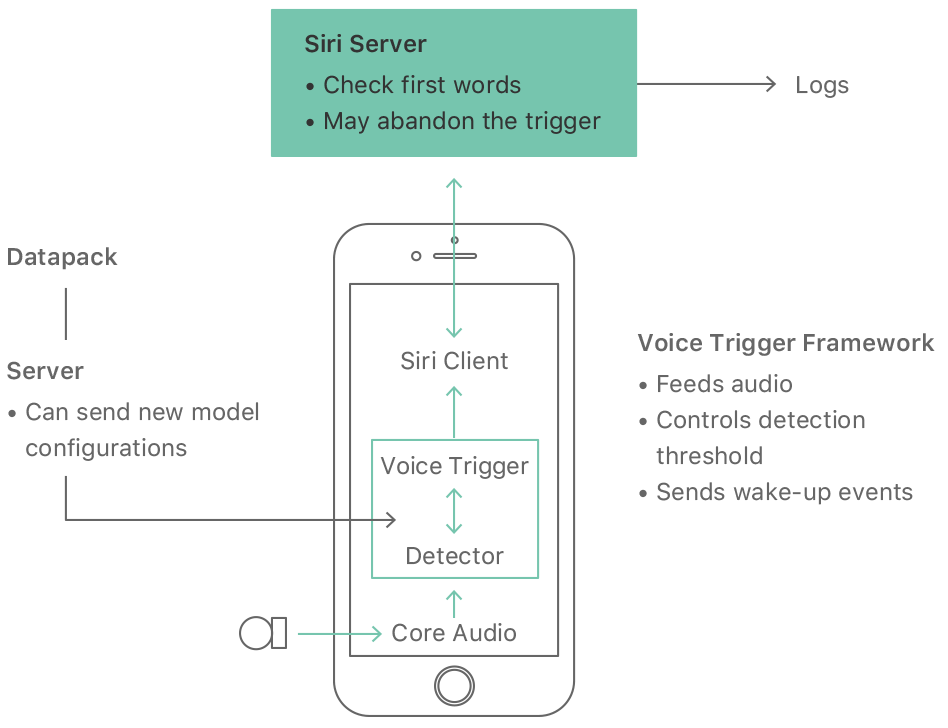
\includegraphics[width = 500]{Dissertation/siri.png}\\
\textit{рис 1. Приклад обробки запиту "Hey, Siri"}


Важливість Siri полягає у тому, що на час запуску технології розпізнавання голосу та розпізнавання мови не були настільки пошиерні, тому, Siri є в певному сенсі першопрохідцем на ринку персональних асистентів.

З іншого боку, її суттєвим недоліком є те, що її функціонал значно обмежений з двох причин. Першою є те, що Siri обмежена тими пристроями, на яких вона запускається - у більшості своїй це телефони та планшети, а не домашні колонки як у конкурентів. Окрім цього, Apple не надає доступу стороннім розробникам доступу до API Siri, через що вона має значно менше функцій, ніж наприклад Alexa.



\subsection{Google Assistant}
Google Assistant[2] - персональний асистент від компанії Google. По суті, це окрема програма, у якій користувач може спілкуватись текстом з асистентом, але Google також випускає асистента у вигляді окремої звукової колонки Google Home разом з озвучкою асистенту та здатністю сприймати голос користувача. 

Серед основних переваг асистента - інтеграція з усіма сервісами Google, що дає змогу поєднувати багато задач у одному асистенті. Крім того, Google Home вміє розпізнавати різні голоси користувачів, що дає можливість персоналізувати взаємодію з ботом навіть у випадку якщо декілька користувачів користуються одним і тим ж е самим пристроєм.

Асистент може робити все на чому спеціалізується Google - шукати на картах, повідомляти останні новини, знаходити інформацію у пошуковики, вмикати музику з Google Music. Також, для створення більш приємного враження від взаємодії з асистентом, у ньому закладено багато сценаріїв та відповідей накшталт "пожартуй" або "розкажи мені казку".

Колонка Google Home також вміє інтегруватись з оточуючими пристроями, такими як датчики та прибори розумного дому, розумні телевізори (через Google Chromecast), тощо.
\subsection{Amazon Alexa}
Amazon Alexa[3] - персональний асистент, інтегрований у аудіопристрої від компанії Amazon. Як і у випадку з Google Assistant, асистент заточений під сервіси компанії, що його розробляє, але бот має і багато інших функцій, серед яких стандартні погода, календар, нагадування, тощо. 

Однією з переваг Alexa є так звані Alexa Skills - Amazon надає API для розробки власних функцій бота, які можна публікувати у спеціальному маркетплейсі. Після цього, будь-який користувач може включити нову функціональність для себе. 

Amazon Lex[4] - технологія розпізнавання мовлення і обробки природньої мови, на основі якої побудована Alexa, є відкритою для розробників. Вони можуть будувати своїх чат-ботів на основі цієї технології.
\section{Огляд існуючих моделей для розв'язування задач}
\subsection{Question-answering моделі}
У 2016 році в [5] було представлено датасет, що складається з 100000 питань з можливими варіантами правильних відповідей по більше, ніж 500 статтям з Вікіпедії. У 2018 році в [6] було оновлено датасет, до нього було додано запитання, що не мають відповіді. 
У 2018 році в [7] було запропоновано модель BERT, що серед інших відомих задач показала два state-of-the-art результати для SQuAD v2.0 і SQuAD v1.1. Наразі, найкращі результати на даних датасетах показують моделі, похідні від BERT - або його модифікації, або використання його у ансамблі з іншими потужними моделями. 
\subsection{Sentiment-analysis моделі}
Є два відомих датасети для оцінювання моделей, призначених визначати тон повідомлення. Першим є збірник відгуків на кінофільми на сайті IMDB, представлений у [8], що складається з 50000 відгуків.  Другим є анотований збірник твітів, що був представлений у [9] та складається з 1,6 міліонів повідомлень з оцінкою тону.
\subsection{Named entity recognition}
Проблема розпізнавання іменованих сутностей є класичною задачею у сфері обробки природньої мови. Вона полягає у знаходженні у тексті власних назв та розпізнавання того, що саме описує власна назва - людину, місце, тощо. \\
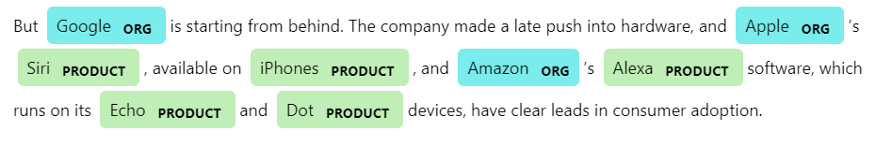
\includegraphics[width = 500]{Dissertation/ner-example.png}\\
\textit{рис 2. Приклад розпізнавання іменованих сутностей.}


У розв'язанні цієї задачі використовуються наступні підходи[10]:
\begin{enumerate}
\item Класичний rule-based підхід.
\item Підходи, що базуються на машинному навчанні.
\item Підходи, що базуються на глибокому навчанні.
\item Комбінації машинного і глибокого навчання. 
\end{enumerate}
Датасетом для перевірки моделей є CoNLL-2003, описаний у [11]. Однією з моделей, що показують state-of-the-art результат, є модель NER DL Annotator [12], представлена у вільнопоширюваній бібліотеці Spark NLP.
\subsection{Spark NLP}
Spark NLP[13] - вільнопоширюванна бібліотека для роботи з природніми мовами. Основною її частиною є натреновані моделі, що мають назву анотатори. Ці моделі можна калібрувати на власних даних та використовувати у так званих пайплайнах.\\
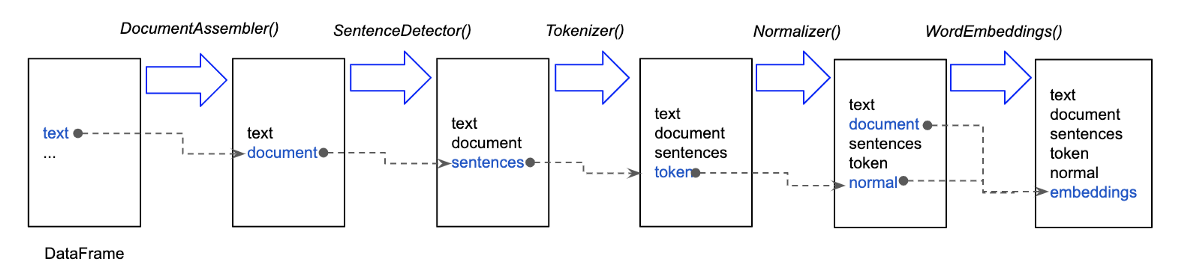
\includegraphics[width = 450]{Dissertation/spark_nlp.png}\\
\textit{рис 3. Демонстрація роботи пайплайну}

Пайплайн - набір моделей, трансформерів та оцінювачів (естіматорів), що послідовно застосовуються до вхідних даних. Spark NLP має кілька заздалегідь натренованих пайплайнів, що маю високі результати у типових задачах обробки природньої мови. 

Для виконання задачі word embeddings, бібліотека використовує натреновану модель BERT, що дає можливість значно покращити результати.

Бібліотека працює на основі двох інших відомих бібліотек - Apache Spark і Apache Spark ML. Оскільки вони підтримуються для мов програмування Scala, Java і Python, то і бібліотека Spark NLP підтримується для усіх цих мов. 

Spark NLP має моделі, натреновані для різних мов, серед яких англійська, французька, італьянська, тощо.
           % Глава 1
\chapter{ТЕОРЕТИЧНИЙ ОГЛЯД ОБРАНИХ ЗАСОБІВ ДОСЛІДЖЕННЯ ТА РОЗРОБКИ }  

\section{BERT}
\subsection{Опис моделі}
BERT - модель, представлена у [3], є однією з найбільш обговорюваних у даний час моделей у сфері обробки природньої мови. Її популярність зумовлена декількома речима. По-перше, модель є надзвичайно універсальною  - вона показує state-of-the-art результати одразу на 11 задачах у сфері обробки природньої мови. По-друге, її легко підтреновувати під конкретну задчу та датасет, що дає можливість використовувати її у різних застосунках. 
\subsection{Як працює модель}
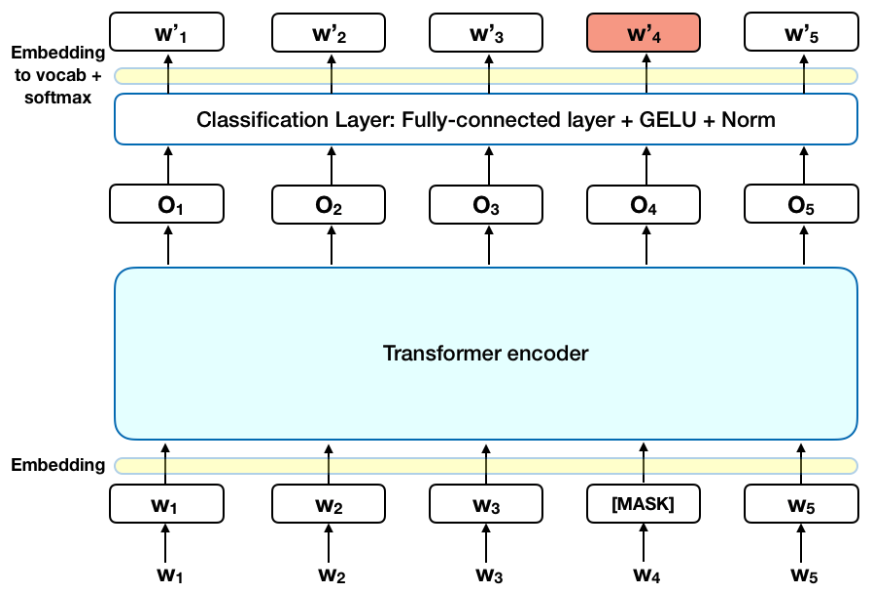
\includegraphics[width=450]{Dissertation/bert_arch.png}\\
\textit{рис. 4. Робота трансформеру.}\\
Основна ідея моделі полягає у тренуванні трансформерів[14] на задачі моделювання мови. Трансформер - це два механізми, один з яких зчитує дані та кодує їх, а інший декодує їх та робить передбачення результату. На відміну від класичних методів роботи з текстами, трансформер не зчитує текст зліва направо, а зчитує все речення разом. Таким чином, ми працюємо з словом та його контекстом, причому контекст слова - це не лише слова перед ним, а й слова після нього. 

Вхідними даними для трансформера є послідовність слів, для яких було пораховано word embeddings[15]. Вихідним значенням є також послідовність векторів, кожний з яких відповідає вхідному слову.

\subsection{Покращення тренування}
Крім трансформерів, BERT також використовує інші підходи для покращення тренування і розуміння контексту слова у реченні. Першим з них є маскування 15\% слів у тренувальних даних. Після трансформації, модель намагається за контекстами сусідніх слів вгадати, яке саме слово було замасковано. 

У тренуванні використовуються пари речень у якості вхідних данних, і модель намагається вгадати друге речення за першим так, ніби це два послідовні речення у одному документі. Під час тренування половина речень є справді послідовними реченнями, а інша половина використовує випадкове речення у якості другого речення.
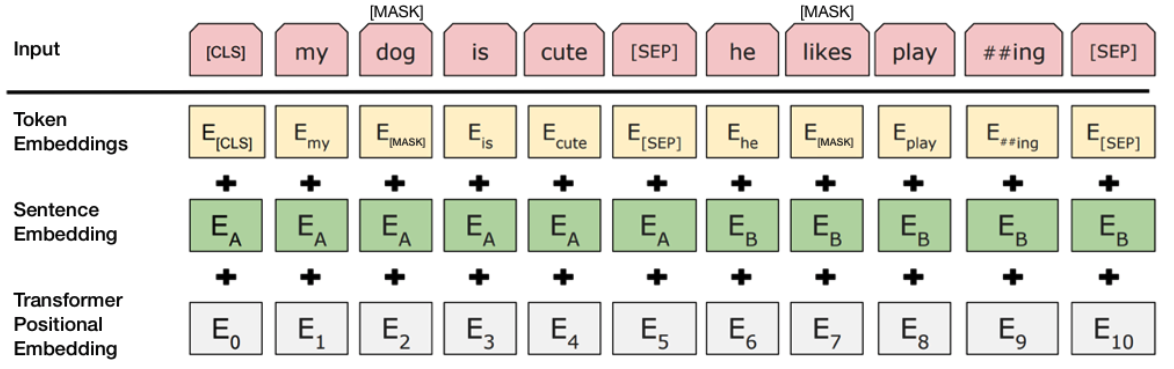
\includegraphics[width = 450]{Dissertation/bert_ex.png}\\
\textit{рис. 5. Як працює тренування на парах речень. }\\
На початок першого речення додається спеціальний токен [CLS], а в кінці кожного речення додаються спеціальні токени [SEP]. Щоб перевірити, чи справді друге речення є пов'язане з першим, ми трансформуємо вхідні данні, та дивимось на значення, що відповідає токену [CLS]. Саме за цим значенням за допомогою функції softmax - це функція $\sigma: \mathbb{R}^{K} \rightarrow \mathbb{R}^{K}$ , що задається формулою
\[
\sigma(\mathbf{z})_{i}=\frac{e^{z_{i}}}{\sum_{j=1}^{K} e^{z_{j}}} \text { for } i=1, \ldots, K \text { and } \mathbf{z}=\left(z_{1}, \ldots, z_{K}\right) \in \mathbb{R}^{K}
\]
 - ми перевіряємо ймовірність того, що ці речення є послідовними.

Ці два підходи поєднується разом під час тренування, з ціллю мінімізувати функцію втрат обох стратегій. Разом, отримуємо модель з понад 375000000 параметрів, що може бути підтренована під різні задачі, пов'язані з природними мовами.
\subsection{Калібрування для інших задач}
 BERT може виконувати багато інших задач у сфері природніх мов [16]. Зазвичай, це досягається додаванням одного додаткового шару у модель. 
 
 Наприклад, задача класифікації текстів вирішується таким саме чином, як і задача розпізнавання наступного речення під час тренування. Додамо спеціальний токен на початку тексту, і за допомогою додаткового шару класифікуємо текст за результатом моделі для цього токену.
 
 Для задачі відповідей на питання, BERT використовує два додаткових вектори, що обозначають початок та кінець відповіді у вихідному тексті.
 
 Для задачі розпізнавання іменованих сутностей, вихідний вектор кожного слова проходить через спеціальний шар-класифікатор. Такий шар класифікує, якому саме типові іменованої сутності  відповідає слово.
 \newpage
\section{Дерево рішень}
\subsection{Опис алгоритму}
Дерево рішень - алгоритм навчання з вчителем, що використовуються у проблемах класифікації. Вперше алгоритм був описаний у [17]. Суть алгоритму полягає у тому, щоб виходячи з тренувальних даних створити бінарне дерево, яке в залежності від деяких параметрів вхідних данних "направляє" їх у ліву чи праву свою гілку. У листках дерева знаходяться відповіді - до якого саме класу належать вхідні дані. \\
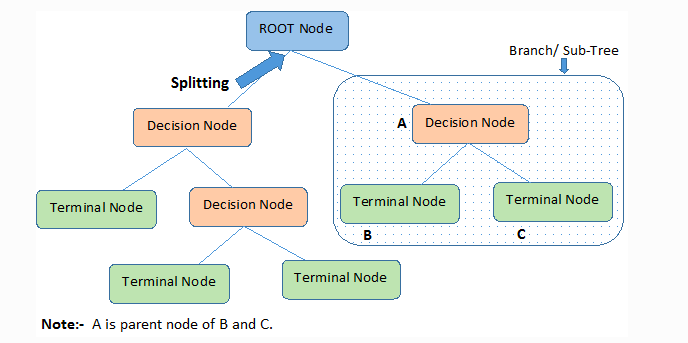
\includegraphics[width = 500]{Dissertation/decision_tree.png} \\
\textit{рис. 6.  Робота дерева рішень}

Перевагою дерева рішень є те, що після тренування, передбачення классу відбувається за час спуску по дереву, тобто 
$\Omega(\log n)$, де n - кількість параметрів моделі. Це дає змогу швидко робити передбачення, використовуючи натреновану модель.
\subsection{Алгоритм побудови}
Дерево рішень будується за наступним алгоритмом[18]. Візьмемо усі тренувальні дані і позначимо їх як кореневу вершину дерева. На кожному кроці роботи алгоритму будемо братий невикористаний параметр з вихідного сету та рахувати його ентропію та додану інформацію. Виберемо параметр, за яким будемо ділити набір даних за допомогою певної метрики. Розділимо набір данних на дві підмножини по цьому параметру та продовжимо рекурсивно роботу алгоритму на цих підмножинах. Будемо продовжувати роботу алгоритму, поки не використаємо усі параметри.

Серед метрик, що використовуються для обрання параметра, за яким будемо ділити, є ентропія, додана інформація, індекс Джині, та додане відношення (описані у [19]).

Ентропія для одного параметру рахується за формулою:
$$
E(S)=\sum_{i=1}^{c}-p_{i} \log _{2} p_{i}
$$, де  S  - поточний стан, a $p_i$ - ймовірність події  i в стані S.
Ентропія для багатьох параметрів рахується за формулою: $$
E(T, X)=\sum_{c \in X} P(c) E(c)
$$, де T - поточний стан, а X- обраний параметр.

Додана інформація - величина, що вказує, наскільки добре даний параметр відділяє дані. 
Вона рахується за наступною формулою: 
$$Information Gain(T,X) = E(T) - E(T, X)$$
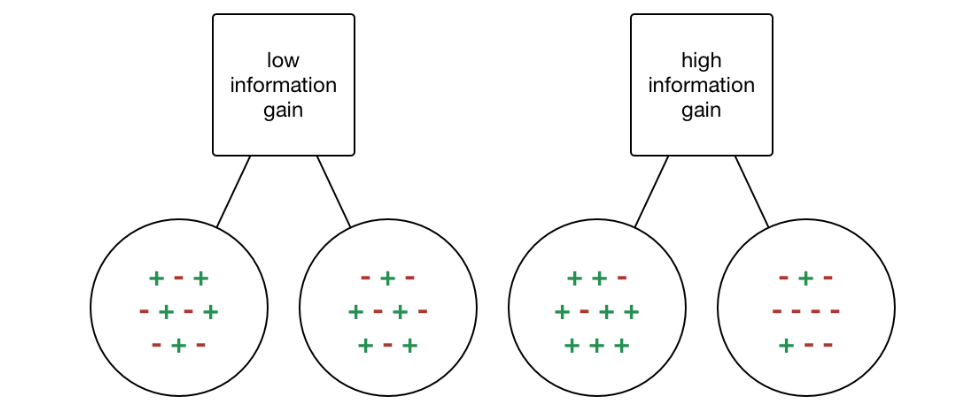
\includegraphics[width=450]{Dissertation/ig.png}\\
\textit{рис 7. Різниця між малою і високою доданою інформацією}

Індекс Джині обчислюється за формулою:
$$
\text {Gini}=1-\sum_{i=1}^{C}\left(p_{i}\right)^{2}
$$
Додане відношення обчислюється за формулою: 
$$
\text {Gain Ratio}=\frac{\text {Information Gain}}{\text {Splittnfo}}=\frac{\text {Entropy}(\text {before})-\sum_{j=1}^{K} \text {Entropy}(j, \text {after})}{\sum_{j=1}^{K} w_{j} \log _{2} w_{j}}
$$



           % Глава 2
\chapter{РЕАЛІЗАЦІЯ ПРОГРАМНОГО ЗАБЕЗПЕЧЕННЯ ДОДАТКУ}

\section{Архітектура додатку}
Введемо наступні поняття:

\begin{itemize}
\item \textbf{Event} (подія) - деяка подія, на яку додаток повинен відреагувати, наприклад - нове повідомлення від користувача.
\item \textbf{Action} (реакція) - реакція додатку на подію, наприклад - збереження нагадування у базу.
\item \textbf{Environment} (середовище) - джерело подій.
\item \textbf{Context} (контекст) - набір даних, об'єднаних за деякою ознакою.
\item \textbf{User} (користувач) - користувач нашого додатку.
\end{itemize}

Побудуємо додаток наступним чином: нехай маємо деякий набір середовищ. Додаток у нескінченому циклі по черзі питає в кожного середовища нові події та реагує на них. Додаток може реагувати на події як окремо, так і будувати певні реакції в залежності від набору подій. 


При першій інтеракції користувача з додатком йому присвоїться унікальний ідентифікатор. Ми зберігатимемо усі дані користувача, що він надав (історію повідомлень, факти надані користувачем, тощо) для того щоб мати можливість персоналізувати його взаємодію з ботом[22]. У подальшому, при визначенні реакції на подію ми враховуватимемо також контекст користувача - тобто сукупність даних про нього.


Таким чином, додаток досить легко розширювати в усі сторони, оскільки усі частини є достатньо незалежними. Якщо ми хочемо додати нову функцію, нам потрібно лише описати подію та відповідну їй реакцію, тобто дію. Якщо ми хочемо зберігати більше даних, нам достатньо лише розширити відповідні контексти. Якщо ми хочемо додати нову платформу, нам достатньо лише вказати яким саме чином ми будемо отримувати повідомлення про дії з неї та задати необхідні реакції. 
\section{Реалізація боту}
Бот складається з чотирьох мікросервісів:
\begin{enumerate}
\item Основний сервіс, написаний мовою Scala - який відповідає за роботу бота
\item Допоміжний сервіс, написаний мовою Scala - використовується разом з SparkNLP для визначення іменованих сутностей у тексті.
\item Сервіс на Python - дає доступ до моделі, що визначає тип повідомлення.
\item Сервіс на Python  - дає доступ до моделі BERT.
\end{enumerate}

Спілкування між сервісами відбувається за допомогою HTTP - повідомлень. Бот також використовує базу даних для зберігання інформації про користувачів. Датасети записуються у текстові файли, що зберігаються на сервері.
\subsection{Месенджер}
У якості месенджера для спілкування з асистентом я обрав Telegram через відносну простоту налаштування та запуску боту. Такий вибір платформи дає можливість в подальшому розширити бота на спілкування не лише текстом, а й за допомогою відеоповідомлень, зображень чи аудіоповідомлень. Для спілкування з API Telegram було обрано існуючу бібліотеку bot4s. 

Відповідно до архітектури, маємо середовище Telegram, яке у якості подій надсилає нам нові повідомлення від користувачів. Бот у свою чергу реагує на них - відповідає іншим повідомленням, оновлює інформацію про користувача, робить запити на зовнішні API чи інші сервіси. Крім того, усі повідомлення логуються у окремий датасет. що дає змогу після анотування використовувати повідомлення для тренування власних моделей.
\subsection{Розпізнавання типу повідомлення}
Для того, щоб якісніше оброблювати повідомлення, необхідно знати, якого саме воно типу.  Введемо 4 наступні типи повідомлень:
\begin{center}
\begin{tabular}{ |c|c| } 
 \hline
Тип повідомлення & Приклад\\
Питання & “What is my age?”\\
Факт & “I am 20 years old”\\
Запит & “Remind me to drink water tomorrow”\\
Інше & “Hello!"\\
 \hline
\end{tabular}
\end{center}\\
\textit{таб. 1 Типи повідомлень.}


Проблема полягає в тому, що не всі користувачі правильно ставлять розділові знаки, тому "what is my age"  має отримати таку саму реакцію від бота, як і "what is my age?". З іншого боку, для запитів, що потребують зовнішні дані (наприклад, "what is the weather today?") цілком нормально мати знак питання, але бути кваліфікованим як саме запит.


Зібравши датасет з повідомлень, та проанотувавши його вручну, натренуємо власний класифікатор повідомлень. Для датасету проводилась така передобробка:

\begin{enumerate}
\item Токенізація (розбиття тексту на слова)
\item Видалення «стоп-слів» (слів, які зазвичай використовуються дуже часто і псують якість моделі)
\item Використання підходу “мішок слів” для переведення слів у числову характеристику.
\end{enumerate}
Найпростіший класифікатор, що тим не менш видає непогану точність, натренуємо наступним чином:

\begin{enumerate}
\item Закодуємо повідомлення за допомогою методу bag of words.
\item Порахуємо кількість знаків запитань у повідомленні.
\item Порахуємо кількість так званих wh-words в повідомленні.
\item Враховуватимемо перше слово у повідомленні окремо.
\item На основі вищевказаних даних натренуємо класифікатор на базі дерева рішень.
\end{enumerate}
На зібраному датасеті отримуємо точність 91.1\%, що є досить непоганою точністю, враховуючи невеликий розмір датасету.

\subsection{Нагадування}
Якщо бот розпізнає повідомлення як запит,  і у тексті міститься ключове слово remind, бот відреагує на повідомлення - перепитає, чи правильно він зрозумів користувача про що і коли потрібно нагадати. Таким чином, збирається датасет нагадувань, на якому можна натренувати модель, що буде відповідати на питання "про що саме потрібно нагадати". Для витягування "тіла" нагадування використовується модель BERT, якій на вхід у якості тексту дається повідомлення, а у якості питання - "What should I remind you about?". На невеликому зібранному датасеті нагадувань BERT дає точність 100\%.\\
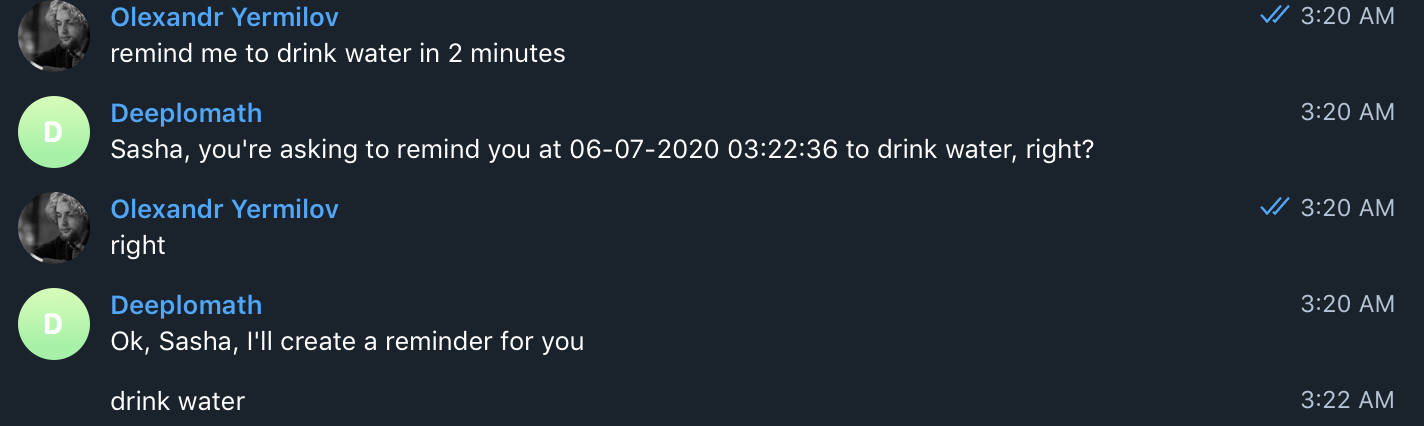
\includegraphics[width=500]{Dissertation/reminder_working.png}.\\
\textit{рис 7. Приклад роботи нагадування.}


Для визначення часу нагадування ми можемо парсити повідомлення користувача, або поєднювати BERT та роботу сервісу. Як і на питання "Про що необхідно нагадати", модель BERT може відповісти на питання "Коли потрібно нагадати?". Але необхідно враховувати, що модель може лише витягнути дані з запиту користувача, і аж ніяк не може дати точний час, у який потрібно нагадати, оскільки модель нічого не знає про те, котра зараз година.\\ 
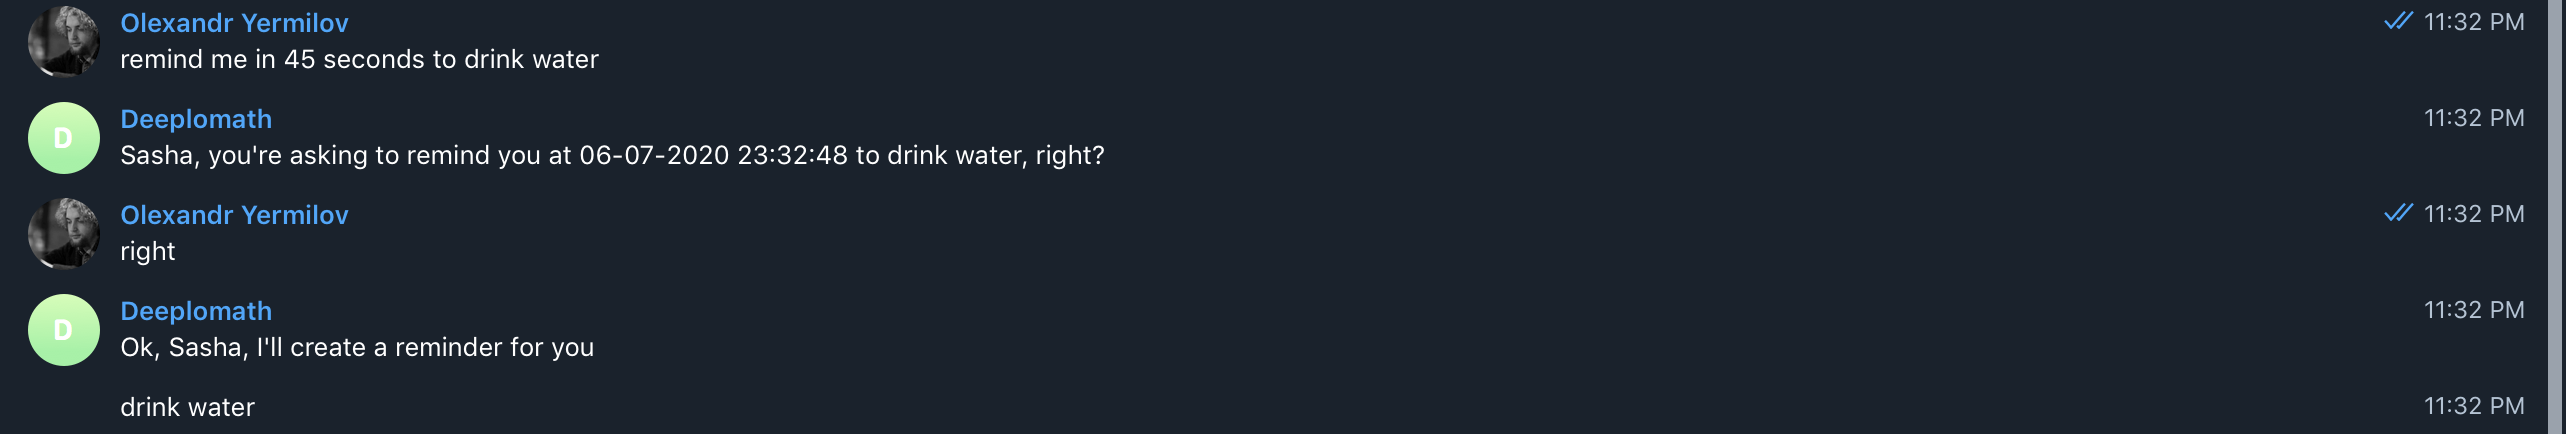
\includegraphics[width=500]{Dissertation/remind_seconds.png}.\\
\textit{рис. 8. Нагадування з іншою одиницею виміру часу.}

\subsection{Запити на зовнішні сервіси}
Робота будь-якого чат-бота сильно залежить від функцій, які він вміє виконувати по запиту користувача. Одним з найкращих способів розширювати його функціональність є інтеграція зі сторонніми API та сервісами, які надають різну інформацію.  

\subsubsection{YahooFinance}
Бот зінтегровано з  API від YahooFinance, що дозволяє дізнаватись ціну акції конкретної компанії. Логіка обробки повідомлення схожа на логіку обробки запиту про нагадування - класифікували повідомлення як запит, за допомогою моделі BERT дістали назву компанії, ціна акцій якої нас цікавить, та виконали запит до стороннього сервісу.\\

\includegraphics[width=500]{Dissertation/stocks_working.png}.\\
\textit{рис 9. Приклад роботи  запиту на сторонній сервіс.}


Крім того, знаючи запити користувача наприклад щодо акцій певної компанії, можемо вважати що він має певний інтерес до неї. Тобто, зберігаючи інформацію такого роду, можна персоналізувати досвід користувача - наприклад, через деякий час запитати, чи цікаво йому знову отримати інформацію про дану компанію. Такого роду інформація зберігається у контексті користувача як інтереси. \\
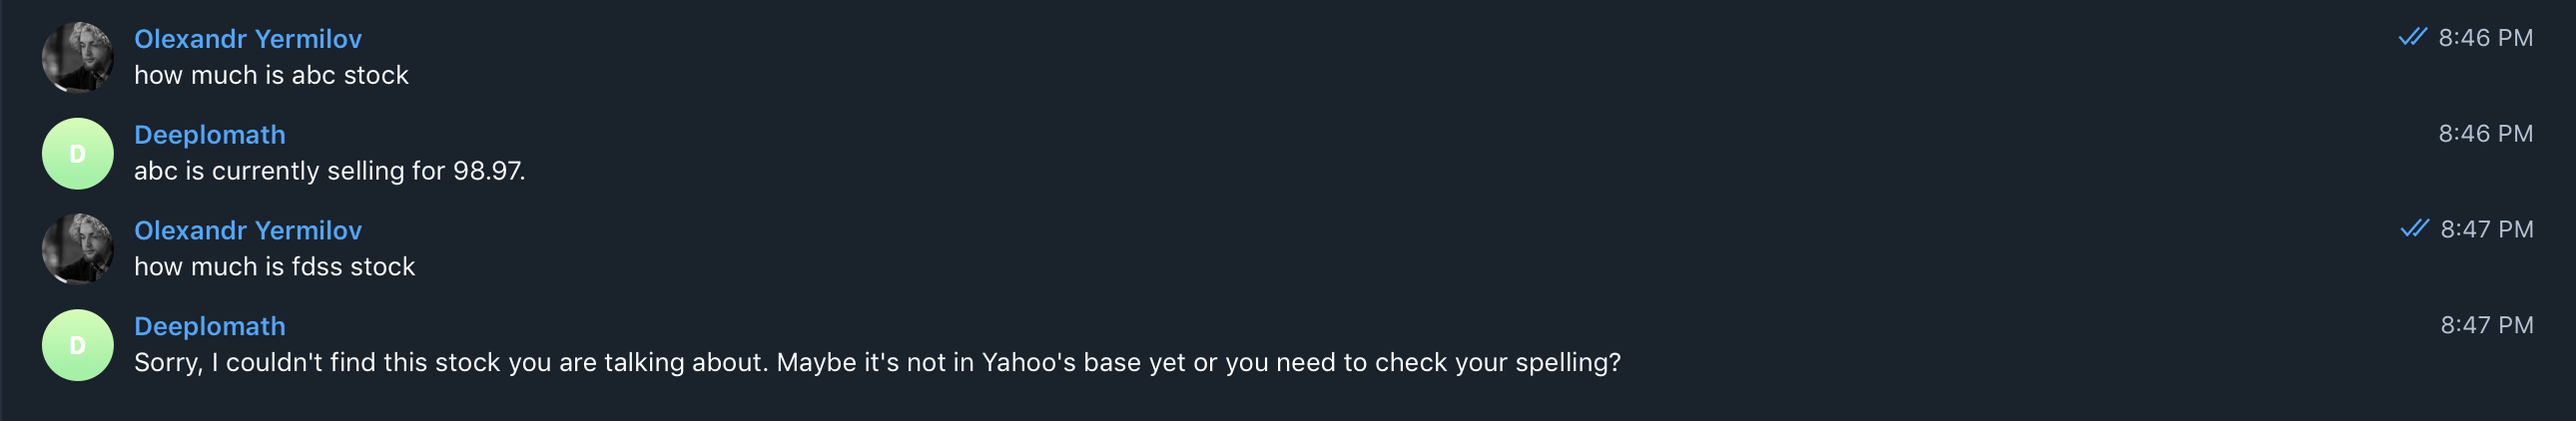
\includegraphics[width = 500]{Dissertation/stocks_not_working.png}\\
\textit{рис. 10 Кілька прикладів роботи з цінами на акції.}


\subsubsection{FoodApi}
Іншим сервісом, обраним для інтеграції з додатком, є сервіс FoodApi. Він дозволяє дізнаватися просту інформацію про їжу - калорії, корисність та склад, тощо. Даний сервіс автоматично відповідає на питання, тому єдине що необхідно зрозуміти - чи повідомлення є запитанням про їжу, чи ні.

\includegraphics[width = 500]{Dissertation/food_api.png}\\
\textit{рис. 11 Приклад запиту про їжу}\\
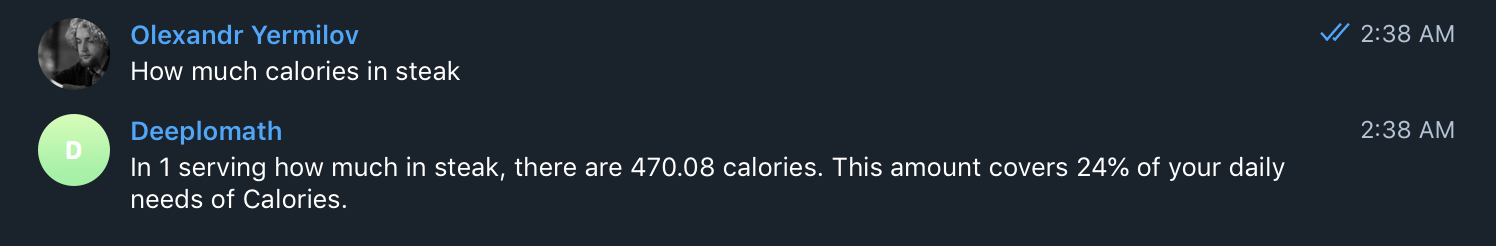
\includegraphics[width = 500]{Dissertation/foodapi2.png}\\
\textit{рис. 12 Запит калорій.}

\subsubsection{Weather API}

Одним із можливо найпопулярніших запитів у чат-ботах є "яка зараз погода?". Для визначення точної погоди необхідно знати точні координати місця, про яке запитує користувач. Для цього можна скористатись стороннім API від Google Maps. 

Для того, щоб дізнатись, про яке саме місце говорить користувач, за звичною схемою запитаємо про це у моделі BERT. Текстом буде питання користувача, у якості питання - "where?" \\
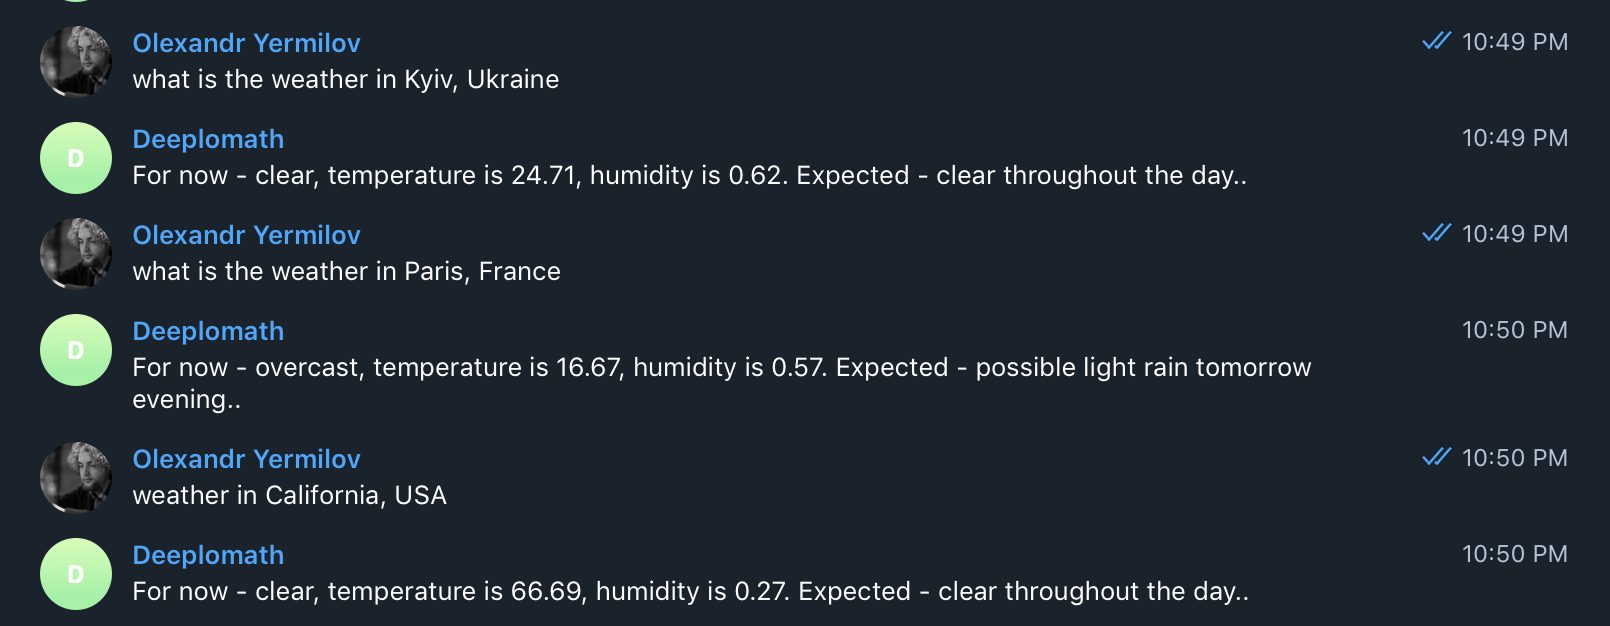
\includegraphics[width = 450]{Dissertation/weather1.png}\\
\textit{рис. 13. Приклад запитів про погоди у різних містах.}

Для визначення погоди скористаємося такоє стороннім API, передавши у якості параметрів довготу та широту місця, про яке запитував користувач. Отримаємо короткий опис теперішнього стану погоди та прогноз на найближчий час. \\
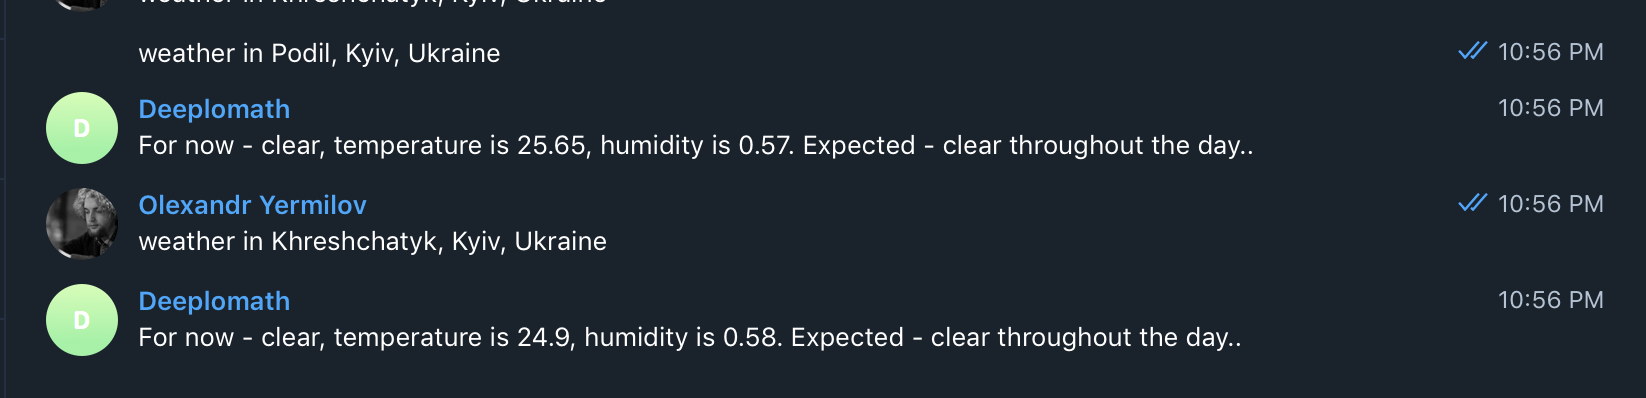
\includegraphics[width = 450]{Dissertation/weather2.png}\\
\textit{рис. 14. Приклад запиту погоди у конкретному районі.}

Як бачимо, завдяки точному визначенню координат можемо отримувати дані про погоду у різних частина Києва.

Телеграм також має підтримку надсилання координат на карті. Скористаємося ними для перевірки погоди за положенням користувача:\\
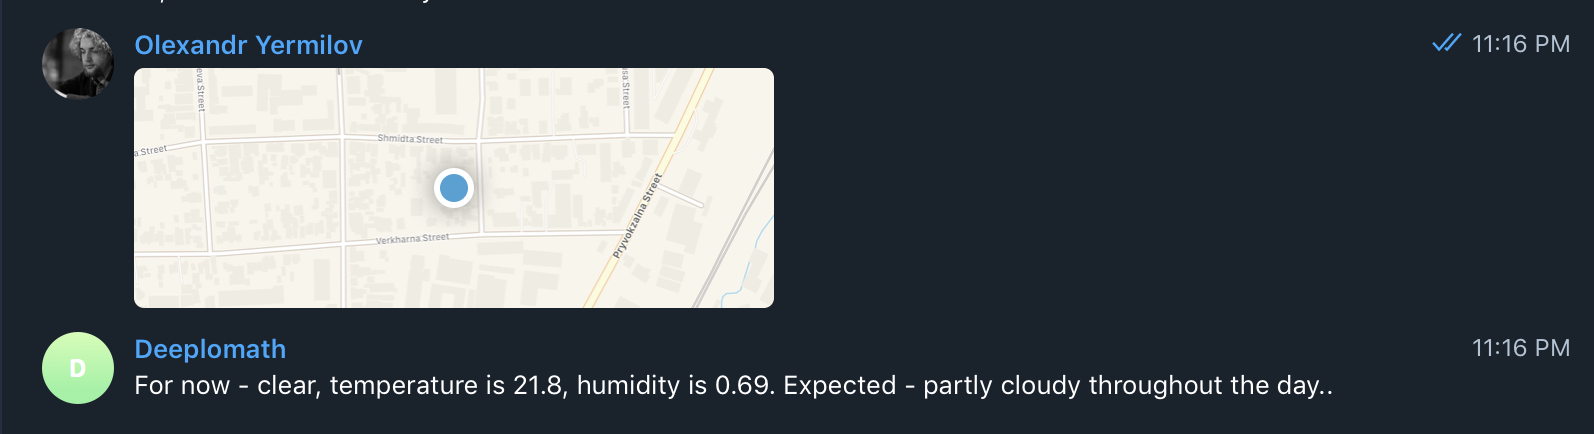
\includegraphics[width = 450]{Dissertation/weather3.png}\\
\textit{рис. 15. Приклад запиту за координатами користувача.}

\subsubsection{COVID API}
Додамо актуальний на даний момент запит - статистика по кількості захворівших COVID-19 у різних країнах. Як зазвичай, скористаємося BERT для визначення країни з запитання користувача за допомогою запитання "where?" та стороннім API для отримання статистики.\\
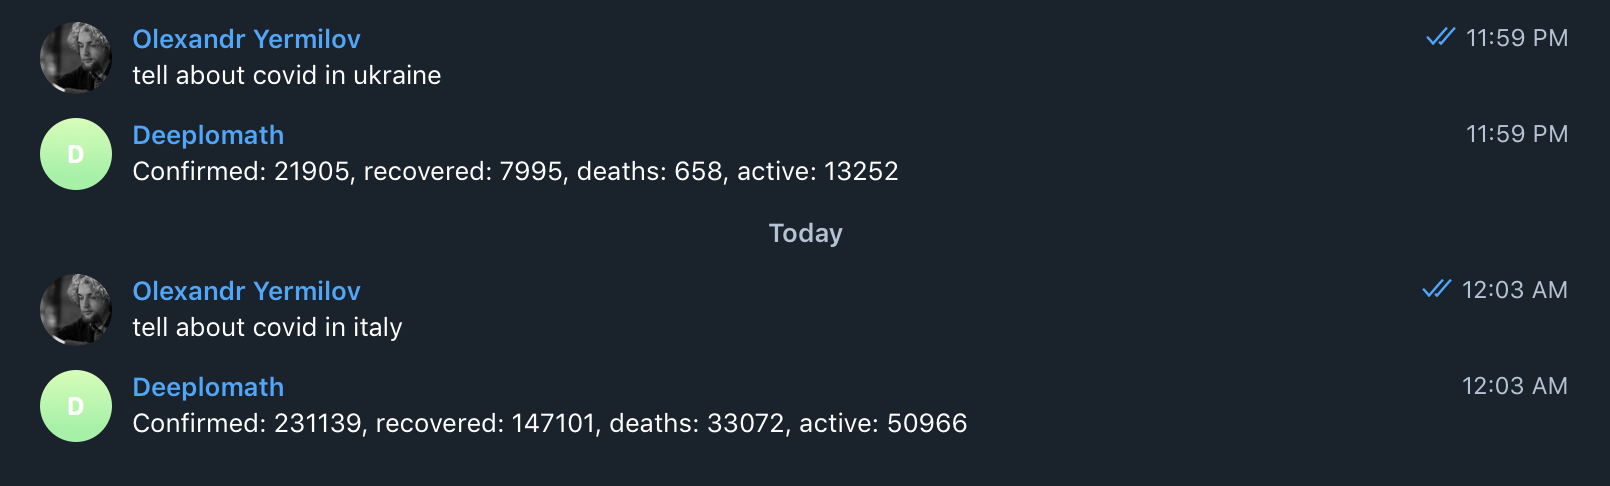
\includegraphics[width = 450]{Dissertation/covid.png}\\
\textit{рис. 16. Приклад запиту про COVID-19}
 

\subsection{Тон повідомлення}
Тон повідомлення є важливою інформацією - якщо користувач протягом останнього часу звучить занадто сумно, це може свідчити про певні проблеми у нього. За допомогою моделі Sentiment Analysis маємо змогу оцінювати кожне повідомлення користувача від -1 до 1, зберігати це значення, після чого у випадку якщо середнє значення перейде за певну межу, можемо зробити висновок про настрій користувача.\\
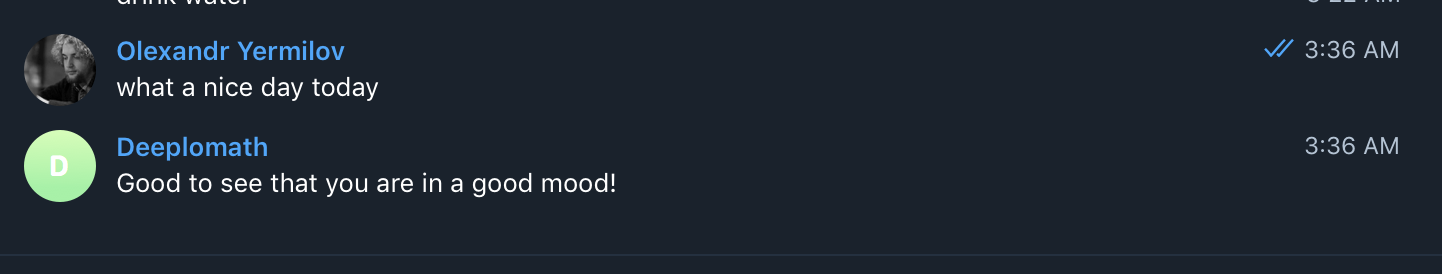
\includegraphics[width=500]{Dissertation/good_sent.png}.\\
\textit{рис. 17. Приклад реакції на гарний настрій користувача.}\\

\includegraphics[width=500]{Dissertation/bad_sent.png}.\\
\textit{рис. 18. Приклад реакції на поганий настрій користувача.}

На прикладах, зображених на рисунках 17 і 18 маємо оцінки тону 0.545 і -0.437 відповідно. Через це, бот реагує відповідним чином.

\subsection{Розпізнавання іменованих сутностей}
Розпізнавання іменованих сутностей є важливою задачею для персонального асистента [21]. На основі іменованих сутностей, що були згадані під час діалогу користувача з чат-ботом, можна дізнаватись про його інтереси, запам'ятовувати факти, що допоможуть у подальших відповідях на питання. \\

\includegraphics[width = 450]{Dissertation/ner_1.png}\\
\textit{рис. 19. Приклад розпізнавання персони}\\

\includegraphics[width = 450]{Dissertation/ner_2.png}\\
\textit{рис. 20. Приклад розпізнавання локації}\\

Для розпізнавання іменованих сутностей використовувалась натренована модель з бібліотеки Spark NLP. Вона використовує word embeddings від моделі BERT. Спілкування між сервісом з Spark NLP та основною частиною боту відбувається за допомогою HTTP запитів.

В залежності від типу іменованої сутності, бот може задавати уточнюючі запитання. Також, бот може зберігати деякі з них як те, що пов'язане з користувачем або є сферою його інтересів.

Для покращення персоналізації, можемо час від часу запитувати про те, що було кваліфіковано як інтерес користувача. Це дозволить збирати більше даих, що в свою чергу дозволить покращувати роботу застосунку.
\subsection{Відповіді на питання}
Будемо зберігати усі повідомлення користувача, що були класифіковані як факти. 
Якщо ми кваліфікували деяке повідомлення від користувача як запитання, скористаємося моделлю BERT для того, щоб дати відповідь на нього. \\
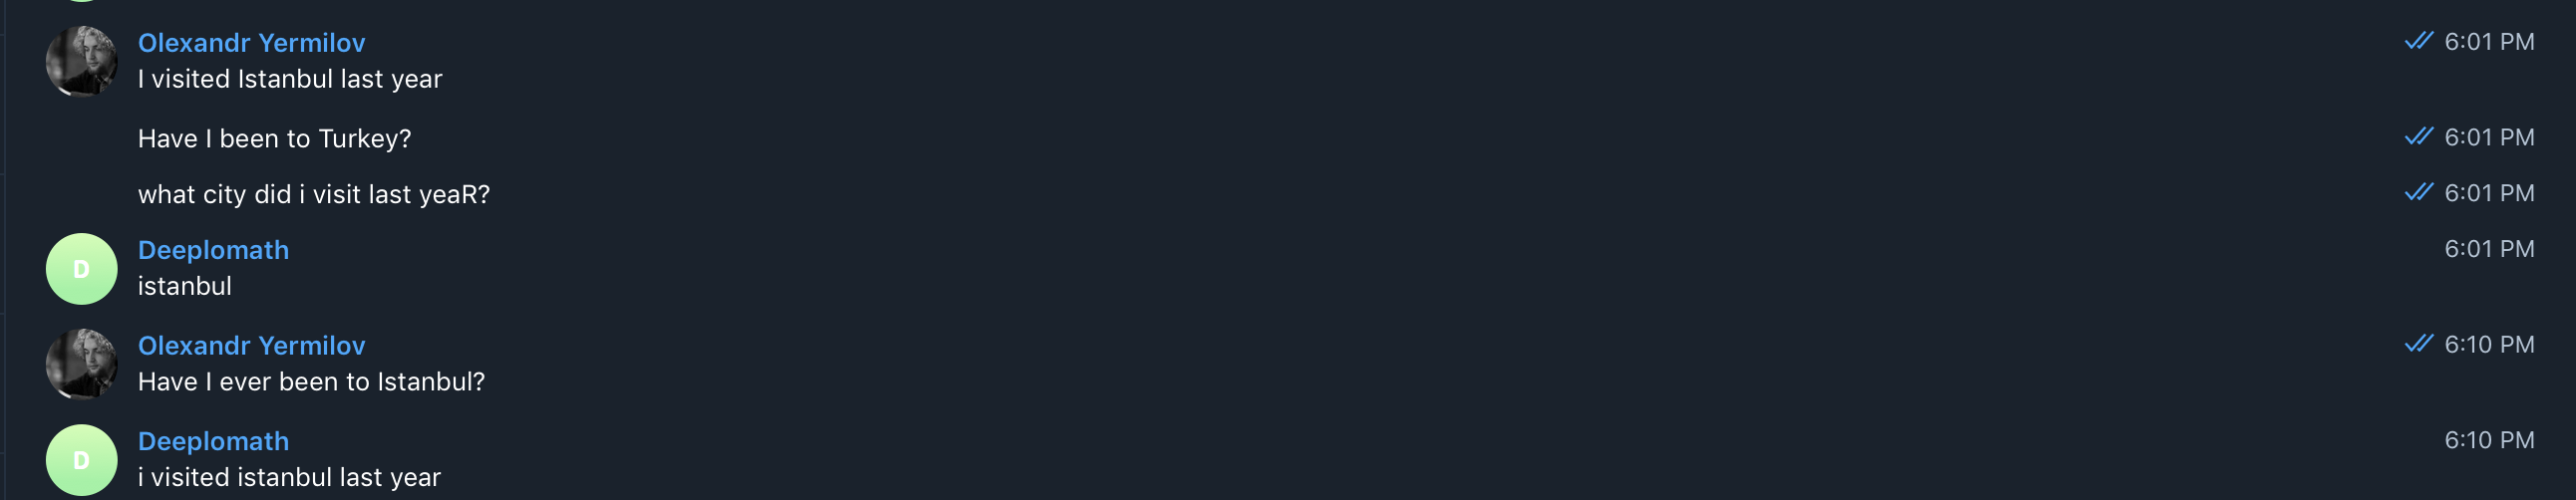
\includegraphics[width = 500]{Dissertation/bert_another.png}\\
\textit{рис 21. Відповіді на запитання користувача}.\\
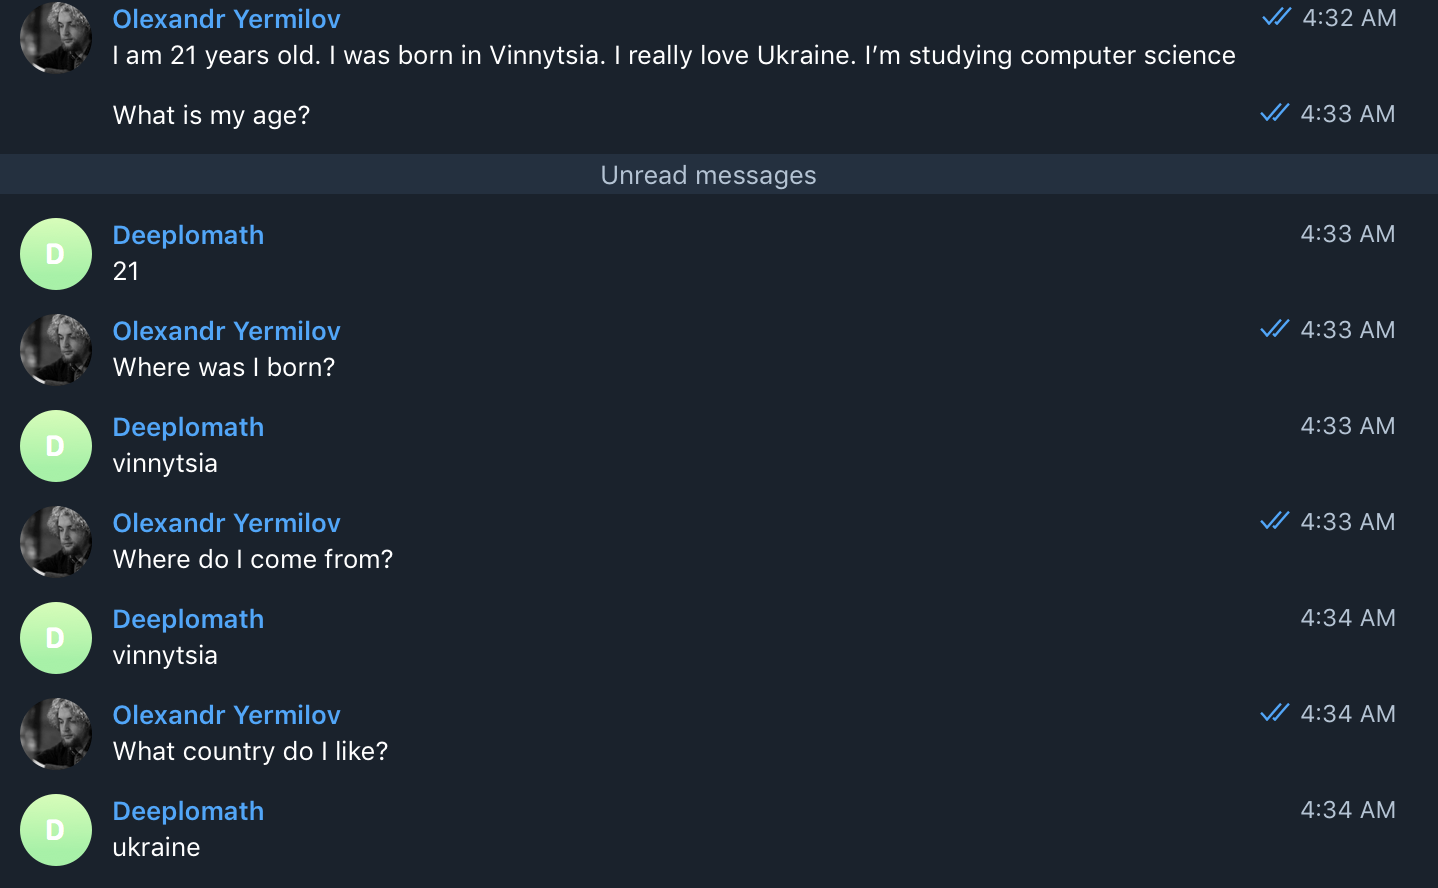
\includegraphics[width=500]{Dissertation/Bert_Example_1.png}.\\
\textit{рис 22. Ще один приклад відповідей на запитання.}

У якості тексту подамо усі повідомлення користувача, що були класифіковані як факти. Окрім того, враховуючи те, що бот має можливість і сам задавати запитання до користувача, ми можемо дописувати до вихідного тексту факти, які ми знаємо про користувача. Якщо збирати інформацію не тільки від користувача, а і від наприклад його гаджету (геолокація, локальний час, тощо) - матимемо змогу додати і ці факти до тексту, яким буде послуговуватись модель при відповіді на питання.

Можемо також враховувати і сфери інтересів користувача, отримані з інших функціональностей бота. Взагалі, модель дуже зручно використовувати для внутрішніх завдань бота - таких, як парсинг запитів користувача, тощо.

Дана модель відповідає в середньому за 0,2 - 0,3 секунди. Такий великий час відповіді пов'язаний з тим, що модель використовується без CUDA, що могло б значно пришвидшити роботу програми. Часом модель значно сповільнюється, на що також необхідно звернути увагу. 
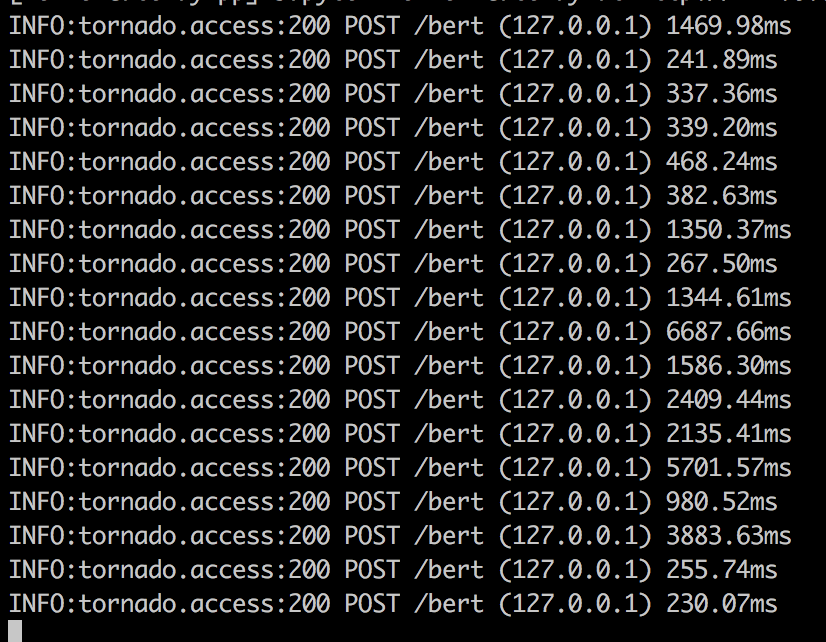
\includegraphics[height = 12cm]{Dissertation/bert_times.png}\\
\textit{рис. 23. Час роботи моделі на деяких запитаннях. }

Також дещо сповільнює роботу той факт, що спілкування між моделлю та серверною частиною застосунку відбувається через HTTP. Використання більш швидкого сервера для Python-частини могло би зменшити час, необхідний на відповідь.

BERT не має власної бази знань, і послуговується лише тим текстом, що був наданий користувачем. Таким чином, модель не може відповісти більшою кількістю інформації, ніж є у повідомленнях користувача. Як приклад, бачимо, що на рисунку 21 модель не може пов'язати Стамбул і Туреччину. Цю проблему можна вирішити якщо до кожного тексту, що надається для відповіді на питання, додавати базовий набір фактів з відкритих джерел про те, про що питає користувач.  Але з іншого боку, збільшення тексту збільшить час на обробку запитання. Також, можемо зробити свою базу знань, що дозволить відповідати на більш загальні питання користувача. В комбінації з розпізнаваннням теми повідомлення, ми можемо підключати бази знань що стоусуються заданої теми - і відповідати на ці питання.

Таку частину боту, що може відповідати на питання можна використовувати для витягнення короткого підсумку користувачем з тексту.




           % Глава 3
\chapter*{ВИСНОВКИ}                       % Заголовок
\addcontentsline{toc}{chapter}{ВИСНОВКИ}  % Добавляем его в оглавление
\section*{Результат}
Було розроблено застосунок, що є простим прототипом персонального асистенту. Застосунок є швидким, має різноманітну функціональність. Окрім виконання функції чат-боту, застосунок вміє збирати датасети для покращення своєї роботи. 

Розроблений застосунок має архітектуру, що спрощує його розширення та збільшення можливих функцій бота. 

Вдалося досягти виконання усіх поставлених задач
\begin{itemize}
\item Бот працює у месенджері Телеграм.
\item Бот має кілька закодованих реплік для простого спілкування з користувачем.
\item Бот може розпізнавати тип повідомлення з точність 91,1\%.
\item Бот вміє робити нагадування, витягуючи точну дату нагадування та тіло нагадування з тексту користувача. Бот збирає окремий датасет для витягування тіла нагадування з вихідного тексту.
\item Бот використовує інформацію з двох сторонніх сервісів. Додавання інших сторонніх сервісів є простою задачею і займає кілька рядків коду.
\item Бот розпізнає теми запитів до нього.
\item Бот може розпізнавати іменовані сутності і запитує більше інформації про них.
\item Бот аналізує загальний тон повідомлення, та має спеціальні репліки, що залежать від настрою повідомлень користувача.
\item Бот може відповідати на запитання, використовуючи одну із найкращих моделей для SQuAD датасету.
\item Бот зберігає усю інформацію надану користувачем
\item Бот збирає два окремих датасети, що можуть допомогти у вдосконаленні його роботи в майбутньому.
\item Більшість відповідей на повідомлення вкладаються у час до 3 секунд. Єдиним повільним місцем, що потенційно може зайняти більше ніж 5 секунд - відповідь на питання по великому тексту.
\end{itemize}

Було зроблено короткий огляд найважливіших задач сфери обробки природньої мови. Описано спосіб оцінювання моделей, що вирішують ці задачі. Використано моделі, що дають найкращі результати у наведених вище задач. На прикладі боту можна побачити, як ці задачі використовуються у реальних застосунках . 

Також зроблено теоретичний огляд моделей та засобів розробки, що використовувались при створенні додатку. Розглянуто роботу моделі BERT, та алгоритм дерев рішень.

Зроблено аналіз застосунків, схожих за метою, наведено їх коротке порівняння та опис переваг.

Користувач може користуватися функцією відповіді на питання у багатьох різних цілях - опрацювання тексту, підготовки до тестів та контрольних, тощо. Цією ж функцією може користуватися бот для більшої точності  та парсингу запитів до нього, тощо.

Дана робота може слугувати базою для майбутніх покращень, що зроблять досвід роботи користувача з ботом більш гладким та персоналізованим.


\section*{Можливі покращення} 
\begin{itemize}
\item Застосування патерну event-sourcing, що полягає у зберіганні всіх подій користувача та побудові інформації про нього як агрегацію усіх збережених подій. Таким чином, ми зможемо змінювати реакції на події все після того, як відбудеться сама подія, що ще більше спростить розширюваність додатку.
\item Для розпізнавання типу повідомлення можна додати парсинг частин мови та частин речення накшталт nltk. Більшість повідомлень складаються не більш ніж з одного речення, а вищевказана класифікація типів повідомлень майже відтворює класифікацію типів речень у англійській мові. А для речень за допомогою парсингу частин речення, мови та побудови дерева залежності слів можна майже з стовідсотковою точністю визначити, чи воно є питанням, чи ні. Скомбінувавши цей спосіб з класифікатором, можна підвищити точність визначення типу повідомлення. 
\item Для пришвидшення швидкості відповіді на питання варто скористатись GPU замість CPU.
\item Для збільшення привабливості користування ботом, необхідно розширювати його функціонал. У цьому можуть допомогти безкоштовні API та вільно поширюванні бібліотеки. 
\item Для збільшення точності класифікації типу повідомлення варто спробувати метод ngram, оскільки він враховує не лише які саме слова наявні у повідомленні, а і їх порядок, що дає змогу краще відрізняти питальні від стверджувальних повідомлень.
\item Для моделей, запущених на Python, можна вдосконалити код, що відповідає на взаємодію з серверною частиною додатку. Якщо використати більш швидкі фреймворки для виставляння REST-endpoint'ів, можна пришвидшити деякі частини застосунку.
\item BERT погано вміє відповідати на питання типу "Так/Ні", але ми можемо передобробити такі питання і заміняти їх на wh-питання, після чого декодувати відповіді у Так чи Ні.
\item Для пришвидшення роботи бота у майбутньому, можна обробляти запити від різних користувачів параллельно. Оскільки в данній моделі бота дані про ріних користувачів не перетинаються, параллельно обробка різних запитів жодним чином не зашкодить цілісності даних.
\item Використання бота у окремому застосунку дозволить отримувати більше данних про користувача.  Наприклад, можна використовувати геолокацію, модель телефона, тощо. Це дозволить значно розширити функції - як приклад, можна створити нагадування, що залежать від локації: "Нагадай мені купити молоко коли я буду в магазині."
\item Використовуючи алгоритми генерації мови, можемо генерувати тексти у випадках, коли не потрібно виконувати запит чи відповідати на питання. Це дасть змогу використовувати бота не тільки як помічника, але і  як співрозмовника. 
\item Можна розпізнавати голосові повідомлення користувача, та в цілому більш широко використовувати можливості платформи Telegram - надсилання відео, зображень, тощо.
\end{itemize}
      % Заключение
\chapter*{\bibname}                       % Заголовок
\addcontentsline{toc}{chapter}{\bibname}  % Добавляем его в оглавление
\begin{enumerate}
    
\item Siri [Електронний ресурс] – Режим доступу до ресурсу: https://www.apple.com/siri/
\item Google Assistant [Електронний ресурс] – Режим доступу до ресурсу: https://assistant.google.com/.
\item Amazon Alexa [Електронний ресурс] – Режим доступу до ресурсу: https://en.wikipedia.org/wiki/AmazonAlexa.
\item Amazon Lex Developer Guide [Електронний ресурс] – Режим доступу до ресурсу: https://docs.aws.amazon.com/lex/latest/dg/lex-dg.pdf.
\item Pranav R. SQuAD: 100,000+ Questions for Machine Comprehension of Tex [Електронний ресурс] / R. Pranav, Z. Jian, L. Konstantin. – 2016. – Режим доступу до ресурсу: https://arxiv.org/abs/1606.05250.
\item Pranav R. Know What You Don't Know: Unanswerable Questions for SQuAD [Електронний ресурс] / Rajpurkar Pranav. – 2018. – Режим доступу до ресурсу: https://arxiv.org/abs/1806.03822.
\item Devlin J. BERT: Pre-training of Deep Bidirectional Transformers for Language Understanding [Електронний ресурс] / J. Devlin, M. Chang. – 2018. – Режим доступу до ресурсу: https://arxiv.org/abs/1810.04805.
\item Learning Word Vectors for Sentiment Analysis [Електронний ресурс]. – 2011. – Режим доступу до ресурсу: https://ai.stanford.edu/ ~amaas/data/sentiment/.
\item Go A. Twitter Sentiment Classification using Distant Supervision [Електронний ресурс] / Alec Go – Режим доступу до ресурсу: https://cs.stanford.edu/people/alecmgo /papers/ TwitterDistantSupervision09.pdf.
\item A Survey on Recent Advances in Named Entity Recognition from Deep Learning models [Електронний ресурс]. – 2018. – Режим доступу до ресурсу: https://arxiv.org/abs/1910.11470.
\item Introduction to the CoNLL-2003 Shared Task: Language-Independent Named Entity Recognition [Електронний ресурс] – Режим доступу до ресурсу: https://www.aclweb.org/anthology/W03-0419.pdf.
\item Named Entity Recognition (NER) with BERT in Spark NLP [Електронний ресурс]. – 2020. – Режим доступу до ресурсу: https://towardsdatascience.com/named-entity-recognition-ner-with-  bert-in-spark-nlp-874df20d1d77.
\item Spark NLP [Електронний ресурс]. – 2017. – Режим доступу до ресурсу: https://databricks.com/blog/2017/10/19/ introducing-natural-language-processing-library-apache-spark.html.
\item Attention Is All You Need [Електронний ресурс]. – 2017. – Режим доступу до ресурсу: https://arxiv.org/pdf/1706.03762.pdf.
\item Mikolov. Efficient Estimation of Word Representations in Vector Space / Mikolov., 2013.
\item BERT Explained: State of the art language model for NLP [Електронний ресурс] – Режим доступу до ресурсу: https: //towardsdatascience.com/bert-explained-state-of-the-art-language-model-for-nlp -f8b21a9b6270.
\item Matching and Prediction on the Principle of Biological Classification, (JRSS, Series C, Applied Statistics, Vol. 8, No. 2, June, 1959, pp. 65-75)
\item Utgoff, P. E. (1989). Incremental induction of decision trees. Machine learning, 4(2), 161–186. doi:10.1023/A:1022699900025
\item Quinlan, J. R. (1987). "Simplifying decision trees". International Journal of Man-Machine Studies. 27 (3): 221–234. CiteSeerX 10.1.1.18.4267. doi:10.1016/S0020-7373(87)80053-6.
\item Spark NLP [Електронний ресурс] – Режим доступу до ресурсу: https://nlp.johnsnowlabs.com/.
\item Mitchell, T.M., Caruana, R., Freitag, D., McDermott, J. and Zabowski, D., 1994. Experience with a learning personal assistant. Communications of the ACM, 37(7), pp.80-91.
\item Mhatre, Namita, Karan Motani, Maitri Shah, and Swati Mali. "Donna interactive chat-bot acting as a personal assistant." International Journal of Computer Applications 140, no. 10 (2016).


\end{enumerate}
       % Список литературы


\appendix
\setlength{\midchapskip}{20pt}
\renewcommand*{\afterchapternum}{\par\nobreak\vskip \midchapskip}
\renewcommand\thechapter{\Asbuk{chapter}}

\include{Dissertation/appendix}        % Приложения

\end{document}
